\documentclass[diss]{template/setrem}

\usepackage[utf8]{inputenc}
\usepackage[table]{xcolor}
\usepackage{multicol}
\usepackage{array}
\usepackage{varwidth}
\usepackage{float}
\usepackage{todonotes}
\usepackage{subfigure}
\usepackage{graphicx,url}
\usepackage{lipsum}

\makeatletter
\g@addto@macro{\UrlBreaks}{\UrlOrds}
\makeatother

\usepackage{setspace}
\usepackage{amssymb}
\usepackage{colortbl}
\usepackage{color}
\usepackage{hyperref}
\usepackage{verbatim}
\usepackage{scrextend}
\usepackage{csvsimple}
\usepackage{glossaries}

\usepackage{listings}
\usepackage{xcolor}
\usepackage{threeparttablex}
\usepackage{lscape}
\usepackage{colortbl}
\usepackage{booktabs}

% Coloca a contagem das figuras sequenciais sem considerar capítulos
\usepackage{chngcntr}
\usepackage{tabularx}
\usepackage{amsmath}
\usepackage{datatool}
\usepackage{seqsplit}
\usepackage[toc,page]{appendix}

% The package option longtable redefines the \cline macro to work around a bug in longtable
\usepackage{longtable}
\usepackage{multirow}
\usepackage{titletoc}

\makeatletter
\def\@cline#1-#2\@nil{%
  \omit
  \@multicnt#1%
  \advance\@multispan\m@ne
  \ifnum\@multicnt=\@ne\@firstofone{&\omit}\fi
  \@multicnt#2%
  \advance\@multicnt-#1%
  \advance\@multispan\@ne
  \leaders\hrule\@height\arrayrulewidth\hfill
  \cr
  \noalign{\nobreak\vskip-\arrayrulewidth}}
\makeatother


\counterwithout{figure}{chapter}
\counterwithout{table}{chapter}

\definecolor{color_keywords}{rgb}{0.0, 0.0, 0.44}
\definecolor{color_mykeyword}{RGB}{10, 100, 112}

\definecolor{myblue}{rgb}{0,0.3,0.9}
\definecolor{mygreen}{rgb}{0,0.6,0}
\definecolor{mygray}{rgb}{0.5,0.5,0.5}
\definecolor{mymauve}{rgb}{0.58,0,0.82}
\definecolor{mygray2}{rgb}{0.2,0.2,0.2}
\definecolor{mygray3}{rgb}{0.4,0.4,0.4}



\lstdefinestyle{mycode}{ %
  %backgroundcolor=\color{yellow!05},   % choose the background color; you must add \usepackage{color} or \usepackage{xcolor}
  basicstyle=\linespread{1}\small,        % the size of the fonts that are used for the code \footnotesize
  %lineskip={-1pt},
  breakatwhitespace=false,         % sets if automatic breaks should only happen at whitespace
  breaklines=true,                 % sets automatic line breaking
  captionpos=t,                    % sets the caption-position to top
  commentstyle=\color{gray!90},    % comment style
%  deletekeywords={...},            % if you want to delete keywords from the given language
  escapeinside={\%*}{*)},          % if you want to add LaTeX within your code
  extendedchars=true,              % lets you use non-ASCII characters; for 8-bits encodings only, does not work with UTF-8
  frame=l,                    % adds a frame around the code (bt,l,r) single
  keepspaces=true,                 % keeps spaces in text, useful for keeping indentation of code (possibly needs columns=flexible)
  keywordstyle=\color{black}\bf,       % keyword style
  language=C++,                     % the language of the code
 % morekeywords={input,output,parallel_activity,stream_producer},            % if you want to add more keywords to the set
  keywordstyle=[2]{\color{blue}\bf},
 % keywords=[3]{serial_in_order, parallel, pipeline, run, add_filter, task_scheduler_init},
 % keywordstyle=[3]{\color{blue!70!green}\bf},
  numbers=left,                    % where to put the line-numbers; possible values are (none, left, right)
  numbersep=5pt,                   % how far the line-numbers are from the code
  numberstyle=\tiny\color{mygray}, % the style that is used for the line-numbers
  rulecolor=\color{black},         % if not set, the frame-color may be changed on line-breaks within not-black text (e.g. comments (green here))
  showspaces=false,                % show spaces everywhere adding particular underscores; it overrides 'showstringspaces'
  showstringspaces=false,          % underline spaces within strings only
  showtabs=false,                  % show tabs within strings adding particular underscores
  stepnumber=1,                    % the step between two line-numbers. If it's 1, each line will be numbered
  stringstyle=\color{red},     % string literal style
  tabsize=1,                       % sets default tabsize to 2 spaces
  title=\lstname                   % show the filename of files included with \lstinputlisting; also try caption instead of title
}

% Negrito no título do listing
\captionsetup[lstlisting]{font={bf},labelfont=bf}

%Ajusta a contagem do listing
\AtBeginDocument{% the counter is defined later
  \counterwithout{lstlisting}{chapter}%
}
\makeatletter
\renewcommand{\l@lstlisting}[2]{%
  \@dottedtocline{1}{0em}{1.5em}{\lstlistingname\ #1}{#2}%
}
\makeatother


\title{Desenvolvimento de um Repositório Institucional de pesquisas acadêmicas baseado em nuvem}
\author{Alf}{Lucas Machado}
%optional
\advisor{Dr.}{LastName}{FirstName}
\advisor{Dr.}{LastName}{FirstName}
\coadvisor{Dr.}{LastName}{FirstName}
\coadvisor{Dr.}{LastName}{FirstName}

% Place where the undergraduate thesis will be made.
\location{Três de Maio}{RS}

% Date of undergraduate thesis development/presentation.
\date{Agosto}{2022}

% Course name - defined in setremdefs.sty.
\course{\ctrc}

% Header image of the cover.
\courseheader{\sistemasinformacaologo[1]}


\docname{Trabalho de Conclusão de Curso do Bacharelado em Sistemas de Informação - Faculdade Três de Maio - SETREM}

% Mostra a lista de tabelas e figuras com os prefixos corretos.
\titlecontents{table}
  [0em]
  {}
  {\tablename\enspace\thecontentslabel:\enspace\enspace}
  {}
  {\titlerule*[.5pc]{.}\contentspage}

\titlecontents{figure}
  [0em]
  {}
  {\figurename\enspace\thecontentslabel:\enspace\enspace}
  {}
  {\titlerule*[.5pc]{.}\contentspage}

\contentsuse{lstlisting}{lol}
\titlecontents{lstlisting}
    [0em]
    {}
    {\lstlistingname\enspace\thecontentslabel:\enspace\enspace}
    {}
    {\titlerule*[.5pc]{.}\contentspage}

\begin{document}


\maketitle
% % folha de rosto
%%%%%%%%%%%%%%%%%%%%%%%%%%%%%%%%%%%%%%%%%%%%%%%%%%%%%%%%%%%%%%%%%%%%%%%%%%%%%%%%
\newpage

{
\begingroup\onehalfspacing
\noindent
\begin{center}
TERMO DE APROVAÇÃO

\vspace{1cm}
\textbf{NAME}\\
\textbf{NAME}

\vspace{1cm}
TITLE HERE
\end{center}

\noindent
Relatório aprovado como requisito parcial para obtenção do título de \textbf{Bacharel em Sistemas de Informação} concedido pela Faculdade de Sistemas de Informação da Sociedade Educacional Três de Maio, pela seguinte Banca examinadora:
\\
\\
\noindent
Orientador: Prof. Name, Dr.\\
Faculdade de Sistemas de Informação da SETREM
\\
\\
\noindent
Name, Dr. \\
Faculdade de Sistemas de Informação da SETREM
\\
\\
\noindent
Name, M.Sc. \\
Faculdade de Sistemas de Informação da SETREM
\\
\\
\noindent
Profa. Vera Lúcia Lorenset Benedetti, M.Sc.\\
Coordenação do Curso Bacharelado em Sistemas de Informação\\
Faculdade de Sistemas de Informação da SETREM.
\\
\\
\vfill
\begin{center}
Três de Maio, 08 de Agosto de 2019.
\end{center}
\endgroup
}

% \begin{agradecimentos}
%   agradeço a todos
% \end{agradecimentos}

% \begin{dedicatoria}
%   dedico a todos
% \end{dedicatoria}

% \keyword{Sistemas de Informação}
% \keyword{Deep Learning}
% \keyword{Agricultura}
% \keyword{Revisão Sistemática da Literatura}
% \begin{resumo}
%   \noindent

%   O resumo vai aqui...

% \end{resumo}


% \keywordenglish{Information Systems}
% \keywordenglish{Deep Learning}
% \keywordenglish{Agriculture}
% \keywordenglish{Systematic Literature Review}
% \begin{abstract}
%   \noindent The abstract goes here ...

% \end{abstract}


% \begin{singlespaced}
%   \listoffigures
% \end{singlespaced}

\begin{singlespaced}
  \listoftables
\end{singlespaced}

% \renewcommand*{\lstlistlistingname}{LISTA DE CÓDIGOS}
% \lstlistoflistings

% \listofmyequations

\begin{listofabbrv}{OR-AC-GAN} % Put the largest abbreviation.
  \setstretch{1}
  \item[APCs] {\emph{Article Processing Charges}}
  \item[BBM] {Biblioteca Brasiliana Guita e José Mindlin}
  \item[BDTC] {Biblioteca Digital de Trabalhos Científicos}
  \item[BOIA] {\emph{Budapest Open Access Initiative}}
  \item[BPMN] {\emph{Business Process Model and Notation}}
  \item[FINEP] {Financiadora de Estudos e Projetos}
  \item[Fiocruz] {Fundação Oswaldo Cruz}
  \item[IBICT] {Instituto Brasileiro de Informação em Ciência e Tecnologia}
  \item[IR] {\emph{Institutional Repository}}
  \item[ISO] {\emph{International Organization for Standardization}}
  \item[NBR] {Norma Brasileira}
  \item[OA] {\emph{Open Access}}
  \item[OAIS] {\emph{Open Archival Information System}}
  \item[OAR] {\emph{Open Access Repositories}}
  \item[OpenDOAR] {\emph{Directory of Open Access Repositories}}
  \item[RDF] {\emph{Resource Description Framework }}
  \item[ROAR] {\emph{Registry of Open Access Repositories}}
  \item[ROARMAP] {\emph{Registry of Open Access Repositories Mandatory Archiving Policies}}
  \item[SETREM] {Sociedade Educacional Três de Maio}
  \item[URI] {\emph{Uniform Resource Identifier}}
  \item[USP] {Universidade de São Paulo}
\end{listofabbrv}

% 
\tableofcontents

\pagestyle{empty}
{
  \chapter*{Introdução} \label{chap:intro}

Os repositórios acadêmicos dentro de instituições de ensino
podem ser vistos como uma ferramenta para a preservação
e propagação do conhecimento, visto que tais repositórios reúnem
o acervo das pesquisas realizadas durante passagem dos acadêmicos
pela instituição, e em teoria disponibilizam fácil acesso a este
material.

Todavia, conforme \cite{PORTO:difusao_cientifica_recortes}
muitas instituições de ciência e tecnologia acabam por não
dispor de uma estrutura profissionalizada de comunicação,
suporte e divulgação dos materiais produzidos, não contemplando
a comunicação em seu organograma funcional, e recorrendo a
improvisações na hora da disponibilização de meios de acesso
a divulgação de seus projetos.

Tendo isto em mente, o tema desta pesquisa surgiu como uma
continuação direta a um projeto de prática profissional
desenvolvido pelo próprio autor, durante o sétimo
semestre da graduação em Sistemas de Informação, na
Sociedade Educacional Três de Maio - SETREM, que possuía
como objetivo analisar o processo de armazenamento e
acesso as publicações realizadas dentro da instituição.

Durante a realização da prática profissional, foi constatado
que a faculdade não possuía um sistema repositório acadêmico
que possibilitasse aos alunos realizar a publicação de seus
artigos e pesquisas. Também foi verificado por meio da aplicação
de um questionário, que mais da metade dos acadêmicos
(cerca de 62,1\% das respostas) apresentavam interesse máximo
em uma escala de 1 a 5, pela utilização de um repositório acadêmico
institucional.

Ao pesquisar sobre repositórios acadêmicos existentes em plataformas
agregadoras como o OpenDOAR\footnote{https://v2.sherpa.ac.uk/opendoar/},
foi constatado que a maioria dos repositórios nacionais utilizam como
base o DSpace, um \emph{software open source} utilizado para a
criação de repositórios acadêmicos institucionais.

Este \emph{software} foi cogitado como um dos principais candidatos
para uma possível implantação dentro da instituição, porem ao buscar
trabalhos relacionados como o de \cite{2019:RodrigoMoreira},
no qual foi relatado que por se tratar de um \emph{software open source},
fica a critério das instituição todas as questões pertinentes a
atualização de versões, personalização, segurança, privacidade dos
dados e \emph{backups} dos arquivos, oque resulta em um ambiente
fragmentado, sendo que algumas instituições utilizam versões antigas
do DSpace, que não funcionam de forma adequada em
dispositivos móveis, conforme relatado no trabalho relacionado
de \cite{2019:FernandesMacedes}.

Tendo como inspiração os tópicos anteriormente citados,
este trabalho de conclusão de curso possui como objetivo a utilização
de tecnologias baseadas em nuvem para realizar a análise e
desenvolvimento de uma plataforma de repositório acadêmico,
que possibilite a interação entre os alunos e orientadores,
englobando o processo de correção e envio de revisões
de publicações dentro da própria plataforma, e que seja uma alternativa
as atuais plataformas de repositórios existentes.

Com a realização deste projeto de pesquisa, buscou-se expor a
importância da utilização de repositórios acadêmicos para realizar
a preservação digital dos materiais produzido, evitando assim a perda
ou esquecimento da produção acadêmica realizada dentro da instituição.
Além de trazer contribuição tanto para os acadêmicos da faculdade SETREM, quanto para outras
instituições que possam optar pela utilização do repositório
acadêmico desenvolvido.

Este trabalho foi estruturado da seguinte forma, no capítulo 1
é abordado o plano de estudo, elencando tópicos como a delimitação
do tema da pesquisa, objetivos, justificativa, metodologia, dentre outros.
No capitulo 2 é apresentado o embasamento teórico e conceitual
visto como necessário para realização deste trabalho.

No capítulo 3 são apresentados os resultados obtidos com a realização desta
pesquisa, protótipos e apresentação do repositório acadêmico proposto.
Em ultima parte, é apresentado a conclusão da pesquisa,
detalhando os objetivos alcançados, validação das hipóteses, dificuldades
e limitações encontradas durante o desenvolvimento, e propostas futuras
de pesquisa.
}
\chapter{Plano de Estudo e Pesquisa} \label{chap:ResearchPlan}




\section{Tema} \label{sec::Theme}
Desenvolvimento de um Repositório Institucional de Periódicos Acadêmicos
baseado em nuvem.

\subsection{Delimitação do Tema} \label{subsec::ThemeDelimitation}

A delimitação do tema se dará como o desenvolvimento de um
repositório institucional de trabalhos acadêmicos, utilizando tecnologias
baseadas em nuvem para realizar o armazenamento e acesso aos dados,
e que envolva o processo de correções e envio de revisões de
publicações dentro da própria plataforma.

O desenvolvimento deste projeto de pesquisa foi realizado durante o período de
maio a julho de 2022, pelo acadêmico Lucas Machado Alf do curso bacharelado
em Sistema de Informação na Sociedade Educacional Três de Maio – SETREM.

\section{Objetivo Geral} \label{sec:objective}

Desenvolver um repositório institucional de periódicos acadêmicos
baseado em nuvem, tendo como objetivo reunir e preservar
as publicações acadêmicas e científicas produzidas em âmbito universitário,
além de unificar o processo de publicações e correções por parte dos orientadores
em uma única plataforma.

\subsection{Objetivos Específicos}
\begin{enumerate}
      \item Explorar ferramentas existentes de repositório acadêmico.
      \item Pesquisar sobre trabalhos e artigos relacionados.
      \item Pesquisar sobre formas de armazenamento de documentos em nuvem.
      \item Investigar mecanismos de busca e análise textual de documentos. (Ex. ElasticSearch e Full Text Search).
      \item Elicitar os requisitos para o desenvolvimento do repositório acadêmico.
      \item Definir as tecnologias que serão utilizadas para o desenvolvimento (Ex: banco de dados, linguagens e frameworks).
      \item Desenvolver uma aplicação web de repositório acadêmico.
      \item Realizar testes no repositório acadêmico desenvolvido, verificando o desempenho da aplicação em relação ao crescimento da quantidade de registros publicados na plataforma.

\end{enumerate}


\section{Justificativa}\label{sec:justification}

O tema desta pesquisa surgiu como uma continuação direta a um projeto
de Prática Profissional desenvolvido pelo próprio autor, durante o sétimo
semestre da graduação em Sistemas de Informação, na Sociedade Educacional
Três de Maio – SETREM, que tinha como objetivo analisar o atual processo
de armazenamento e acesso as publicações produzidas dentro da faculdade,
e realizar a representação gráfica dos processos por meio de diagramas BPMN
(\emph{Business Process Model and Notation}).

Conforme o próprio autor, durante o desenvolvimento da pesquisa foi constatado que a faculdade
não possuía um sistema de repositório acadêmico que possibilitasse aos
alunos realizar a publicação de seus artigos, práticas profissionais,
interdisciplinares, TCCs e demais pesquisas realizadas na instituição.
Também foi verificado por meio da aplicação de um questionário, que
mais da metade dos acadêmicos (cerca de 63,1\% das respostas) apresentavam
interesse máximo em uma escala de 1 a 5, por um repositório acadêmico
institucional.

Ao pesquisar sobre repositórios acadêmicos existentes em plataformas
agregadoras como o OpenDOAR\footnote{https://v2.sherpa.ac.uk/opendoar/}, foi constatado que a maioria dos repositórios
nacionais utilizam como base o DSpace, um \emph{software open source}
escrito em Java para criação de repositórios acadêmicos institucionais,
sendo minoria as instituições que utilizam um sistema de repositório
institucional diferente deste.

No trabalho relacionado de \cite{GarciaRodrigoMoreira2019DdnB} é possível
verificar que por se tratar de um \emph{software open source},
fica a critério das instituições as questões pertinentes a personalização
do DSpace, segurança e privacidade dos dados, \emph{backup} dos arquivos,
e a realização das atualizações de versão, o que resulta em um ambiente
fragmentado onde algumas instituições utilizam versões antigas do \emph{software},
que por exemplo não funcionam de forma adequada em dispositivos móveis como
relatado no trabalho relacionado de \cite{FernandesMacedes:2018}.

Possuindo como inspiração os tópicos anteriormente citados,
este trabalho de conclusão de curso possui como objetivo e principal
contribuição cientifica, a utilização de tecnologias baseadas em
nuvem para realizar a análise e desenvolvimento de uma nova plataforma
de repositório acadêmico, que possibilite a interação entre os alunos
e orientadores, englobando o processo de correção e envio de revisões
de publicações dentro da própria plataforma, e que seja uma alternativa
as atuais plataformas de repositórios existentes.

Com a realização desta pesquisa, buscou-se trazer contribuição
tanto para os acadêmicos da faculdade SETREM, quanto para outras
instituições que possam optar pela utilização do repositório
acadêmico desenvolvido. Também houve o proposito de expor a
importância da utilização de repositórios acadêmicos para realizar
a preservação digital dos materiais produzido, evitando assim a perda
ou esquecimento da produção acadêmica e cientifica realizada dentro
da instituição.

Com o aprendizado adquirido durante o desenvolvimento deste trabalho
de conclusão de curo, foi possível realizar o aprofundamento do
conhecimento nas áreas de tecnologia da informação, nuvem computacional,
repositórios acadêmicos, gestão de conhecimento, linguagens de programação
e demais tecnologias utilizadas durante o desenvolvimento da pesquisa.

\section{Problema} \label{sec::Problem}

Como problema, foram ressaltados dois pontos principais que motivaram a
escolha do tema desta pesquisa, sendo o primeiro a necessidade de reunir
as publicações acadêmicas produzidas dentro de instituições de ensino
superior em um repositório institucional, que forneça rápido acesso às
publicações científicas produzidas dentro da instituição, tanto de forma
interna para os estudantes da instituição, quanto de forma externa caso
a instituição opte por disponibilizar o seu acervo de forma pública.

Já o segundo ponto, envolve a forma como ocorre o processo de publicação,
correção e revisão por parte dos orientadores, que em geral envolve a
troca de vários emails entre os orientadores e os orientandos,
processo o qual poderia ser melhorado por meio de um repositório
acadêmico que suporte um esquema de publicação de revisões e correções.

Levando em consideração estes pontos, o problema desta pesquisa
foi definido como: Como projetar um repositório de trabalhos
acadêmicos baseado em serviços de nuvem, que envolva o processo
de correções e envio de revisões das publicações dentro
da própria plataforma?

\section{Hipóteses} \label{sec::Hypothesis}
\begin{enumerate}
      \item O recurso de Full Text Search do banco de dados PostgreSQL
            pode ser utilizado como uma alternativa viável para realizar
            as consultas por publicações dentro do repositório acadêmico
            (menos de 5 segundos por consulta), mesmo em bases de dados
            com mais de 30 mil publicações.

      \item O processo desenvolvido para extração do texto das publicações
            para pesquisa e indexação é rápido o suficiente para não
            necessitar de processamento em segundo plano (menos de 5 segundos),
            mesmo em publicações com mais de 200 páginas.

      \item É possível manter um ambiente em nuvem contendo os serviços
            de backend, frontend, banco de dados e armazenamento das
            publicações em nuvem, com um orçamento máximo de R\$ 500,00
            por mês.

\end{enumerate}


\section{Metodologia} \label{sec:Methodology}

Conforme \citep[p. 15]{LOVATO:metodologia} a metodologia de pesquisa
consiste em um ramo da filosofia da ciência, que estuda os métodos que
os cientistas podem utilizar para chegar nos resultados de seus estudos.
Em outras palavras, tem como objetivo estudar os métodos que visam
conduzir um aumento do conhecimento sobre o tema pesquisado, preocupando-se
com o raciocínio, procedimentos e técnicas que podem ser utilizadas para
dar credibilidade aos resultados.

\subsection{Abordagem}

Os métodos de abordagem segundo \citep[p. 29]{LOVATO:metodologia} podem ser
divididos em dois grupos, o primeiro consiste no tipo de raciocínio que
é utilizado para se chegar aos resultados e conclusões. Já o segundo
se relaciona com a utilização, ou não, de análise numérica e estatística.

Segundo o mesmo autor, a abordagem quantitativa é utilizada quando
as conclusões são obtidas por meio de um conjunto de dados numéricos
e analise estatística, busca compreender melhor situações onde é possível
estabelecer relação entre variáveis, correlações ou causa-efeito.

Já segundo \cite{GIL:metodologia} a abordagem dedutiva, conforme a definição clássica,
é o método em que se parte de um conceito geral, onde parte dos
conceitos são conhecidos como verdadeiros ou falsos, e se chega
a uma conclusão particular, por meio da aplicação da lógica.

Para o desenvolvimento deste trabalho, foram utilizadas as abordagens
dedutiva e quantitativa, respetivamente a primeira abordagem foi utilizada
de forma a utilizar o raciocínio logico sobre pesquisas e repositórios
acadêmicos já existes, para melhor compreender o escopo da pesquisa,
e assim propor soluções mais adequadas ao problema.

Já a segunda abordagem foi utilizada para mensurar e analisar
os dados numéricos referentes ao tempo de consultas e arquivamento
das publicações no repositório acadêmico proposto, além dos
custos envolvendo o armazenamento das publicações em nuvem.

\subsection{Procedimentos}

São apresentados neste tópicos os procedimentos utilizados
durante a realização deste trabalho, como a pesquisa bibliográfica e
o método de pesquisa ação.

\subsubsection{Pesquisa Bibliográfica}

Conforme \citep[p. 183]{LAKATOS:metodologia}, a pesquisa bibliográfica
abrange toda a bibliografia que se refere ao tema da pesquisa,
incluindo desde publicações avulsas, boletins, jornais, revistas,
livros, monografias, até meios de comunicação via rádio,
gravações e filmes, tendo como finalidade realizar o contanto
entre o pesquisador e o material já existente sobre o tema pesquisado.

Este procedimento foi utilizado por meio da realização de pesquisas
em livros, artigos e revistas, com a finalidade de se obter
conhecimentos sobre o tema pesquisado, e outros sistemas
já existentes com propósitos semelhantes.

\subsubsection{Pesquisa Ação}

Como elicitado por \citep[p. 45]{LOVATO:metodologia}, a pesquisa ação
diferente de outras abordagens em que o principal
embasamento consiste na literatura, o problema é real, e não existe
um plano previamente definido e inflexível, mas sim um refinamento
contantes entre planejar, agir avaliar e refletir.

Por se tratar do desenvolvimento de um \emph{software}, o procedimento
de pesquisa ação foi utilizado na forma da pesquisa,
aplicação e avaliação de tecnologias existentes, e que possam
ser utilizadas durante o desenvolvimento do repositório
acadêmico proposto.

\subsection{Validação das Hipóteses}

Durante a elaboração do presente trabalho, foram elencadas
três hipóteses, sendo a  primeira "O recurso de Full Text
Search do banco de dados PostgreSQL pode ser utilizado como
uma alternativa viável para realizar as consultas por publicações
dentro do repositório acadêmico (menos de 5 segundos por consulta),
mesmo em bases de dados com mais de 30 mil publicações".
Esta hipótese pode ser validada por meio da preparação de uma base
de dados de testes, que contenha mais de 30 mil publicações, e
em seguida, realizar uma mesma consulta diversas vezes, realizando
a média de tempo de execução.

A segunda hipótese é apresentada como "O processo desenvolvido
para extração do texto das publicações para pesquisa e indexação
é rápido o suficiente para não necessitar de processamento em
segundo plano (menos de 5 segundos), mesmo em publicações com mais
de 200 páginas". Esta segunda hipótese pode ser validada por meio
de um teste de desempenho, que consiste realizar a publicação de uma
mesma publicação com mais de 200 páginas diversas vezes, e mensurar
o tempo médio para conclusão do processo.

Já a terceira hipótese, consiste em "É possível manter um ambiente
em nuvem contendo os serviços de backend, frontend, banco de dados
e armazenamento das publicações em nuvem, com um orçamento máximo
de R\$ 500,00 por mês". Esta hipótese pode ser validada por meio
da comparação dos preços de diferentes provedores de nuvem, com
base nos requisitos mínimos estipulados para o repositório
acadêmicos proposto.

\subsection{Técnicas}

Conforme \citep[p. 174]{LAKATOS:metodologia} as técnicas podem
ser definidas como um conjunto de procedimentos que servem a
uma ciência ou arte, sendo utilizados para trazer tais
conceitos a parte prática, tendo em mente que toda ciência utiliza
de incontáveis técnicas para a obtenção de seus resultados.

Durante o desenvolvimento desta pesquisa, por se tratar do
desenvolvimento de um \emph{software}, foi utilizado da técnica
de prototipação de telas por meio de \emph{mockups} realizados
com a ferramenta Figma\footnote{https://figma.com/}.

Em tradução livre de \cite{uzayr:mockups} um \emph{software mockup}
consiste em um desenho de uma página ou aplicação web,
que é desenvolvida para trazer vida a uma ideia, permitindo
que um designer possa examinar como diferentes elementos visuais
trabalham juntos. Os \emph{mockups} também permitem que as partes
interessadas ou \emph{Stakeholders} do projeto possam verificar como a
interface irá parecer, enquanto sugerem mudanças
apropriadas em relação a cores, imagens e estilos.

Também foram utilizadas as técnica de modelagem ER (Entidade Relacionamento)
por meio da ferramenta pgModeler\footnote{https://pgmodeler.io/} para
o desenvolvimento do banco de dados, e testes para verificar o funcionamento
do \emph{software} desenvolvimento.

\section{Orçamento} \label{sec:budget}

%table example

\section{Cronograma de Atividades} \label{sec:schedule_activities_table}

%table example
% Chapter 2

\chapter{Fundamentação Teórica}\label{chap:background}

\section{Gestão do Conhecimento}\label{sec:business}
\subsection{Gestão do Conhecimento Científico}
\subsection{Repositórios Institucionais}
\subsection{Padrão Dublin Core para metadados descritivos}
\subsection{Open Archival Information System (OAIS)}

\section{Ferramentas utilizadas}\label{sec:fundamental}
\subsection{Cloud Computing}
\subsection{Cloud Object Storage}
\subsection{Microsoft .NET}
\subsection{ReactJS}
\subsubsection{Vite}

\subsection{PostgreSQL}
\subsubsection{FullText Search}
\subsubsection{GIN Index}

% \section{Sistemas Relacionados}\label{sec:rs}
% \subsection{DSpace}
% \subsection{Open Journal Systems}
% \subsection{ResearchGate}

\section{Trabalhos Relacionados}\label{sec:rw}

São apresentados neste tópico, os trabalhos relacionados, que possuem
algum ponto em comum com o que se quer realizar no presente projeto.
Pretendesse aqui, identificar estes pontos, e compará-los com a proposta deste projeto.

\subsection{BDTC - Uma Biblioteca Digital de Trabalhos Científicos com Serviços Integrados}

O trabalho desenvolvido por \cite{CERVI:bdtc}, possui como premissa a apresentação
de uma proposta de biblioteca digital de trabalhos científicos, que foi denominada como
BDTC, que possui como objetivo prover o suporte a três pontos fundamentais:
auto-arquivamento do conteúdo, extração de metadados e busca de similaridade.

Como um dos principais diferenciais, foi desenvolvido um mecanismo de
busca por similaridade para as pesquisas realizadas na BDTC,
que permite ao usuário encontrar trabalhos relacionados, mesmo que
parte da palavra pesquisada não seja exatamente igual ao conteúdo presente
no documento.

Para o desenvolvimento deste mecanismo de busca, foi utilizado
um recurso denominado \emph{n-gram}, que permite quebrar uma palavra em
conjuntos de letras de tamanhos variados, é retratado como exemplo o
\emph{3-gram} do termo "Juci", que podem ser quebrado em dois conjuntos de 3
letras, ou seja, \emph{"Juc"} e \emph{"uci"}.

Estes conjuntos são armazenados em uma tabela de índices no banco de
dados, de forma que ao realizar uma consulta a partir de uma palavra,
o sistema retorna todos os trabalhos que contenham algum dos conjuntos
de letras que compõem a palavra pesquisada.

Em relação com o presente projeto, pode ser realizado uma comparação com
a forma como o mecanismo de busca foi desenvolvido na BDTC. Ao envés de
utilizar o recurso de \emph{n-gram}, o sistema proposto neste projeto utilizara
o recurso de \emph{tokenization} presente na ferramenta de \emph{Full Text Search} do
banco de dados PostgreSQL, que possui um resultado final semelhante, porem não
idêntico, visto que o \emph{tokenization} remove o gênero das palavras,
os espaços em branco, palavras comuns e palavras que não são consideradas relevantes.

\subsection{Desenvolvimento da nova Biblioteca Digital da Biblioteca Brasiliana USP: Relato de Experiência}

O relato de experiência desenvolvido por \cite{GarciaRodrigoMoreira2019DdnB}
apresenta o desenvolvimento da na nova plataforma de Biblioteca Digital da
BBM, a Biblioteca Brasiliana Guita e José Mindlin, em forma de retrospectiva
desde o projeto-piloto, relatando os principais problemas, êxitos
e desafios encontrados durante o desenvolvimento do projeto, que envolvia
a digitalização e desenvolvimento de uma coleção digital para a biblioteca.

A Biblioteca Brasiliana Guita e José Mindlin foi inaugurada em março
de 2013, sendo um órgão e entidade acadêmica da Pró-Reitoria de Cultura
e Extensão da USP (Universidade de São Paulo). Este biblioteca envolve o
projeto Brasiliana USP, que foi iniciado em 2005, e tem como objetivo
abrigar a coleção Brasiliana, doada por José Mindlin. Dentro do escopo
deste projeto, em 2008 é iniciado o projeto-piloto da Biblioteca
Brasiliana Digital, que visa a preservação do acervo e democratização
do acesso ao material.

Para o desenvolvimento da biblioteca digital, foi optado por realizar uma
customização do sistema DSpace, um \emph{software open source} de repositório
digital, com recursos como o Djatoka (servidor de imagens) e visualizadores
de livros como IIPImage e BookReader.

Como principais problemas e êxitos, foi ressaltado a forma como as customizações
foram realizadas no DSpace, sendo muitas delas realizadas diretamente no código fonte
do programa, tornando extramente difícil ou até impossibilitando a atualização
para novas versões da plataforma. Resultado em inconsistências na
visualização dos documentos digitalizados, lentidão do sistema, dentro outros
problemas que vieram a surgir ao longo do tempo.

Além disto, também foi relatado a rotativada das equipes como um fator de impacto
para a continuidade do desenvolvimento da biblioteca, que em sua
maioria era constituída por bolsistas, estagiários e poucos profissionais
terceirizados contratados por tempo determinado. Também foi constatado
que as máquinas digitalizadoras adquiridas para a biblioteca não eram
adequadas para o manuseio dos documentos do acervo, visto que os documentos
eram obras raras, e que necessitavam de diversos cuidados para a preservação
e conversação do material.

Com o tempo parte dos problemas foram resolvidos, sendo até adquirido novas
maquinas digitalizadoras, mais modernas e adequadas para o manuseio do material
bibliográfico.

Comparando o trabalho relacionado com o presente projeto de pesquisa,
é possível ressaltar que o atual projeto não tem como intenção a digitalização
de um acervo físico, porem o sistema DSpace que foi utilizado no trabalho
relacionado foi identificado como um sistema muito popular para o desenvolvimento
de repositórios acadêmicos e bibliotecas digitais de universidades, sendo
possível utilizar a experiência adquirida na implantação desse sistema durante
o desenvolvimento do repositório acadêmico proposto.

\subsection{Classificação facetada: proposta de categorias fundamentais para organizar teses e dissertações em uma biblioteca digital}

O artigo desenvolvido por \cite{PereiraClaytonMartins2021Cfpd} tem como
proposta a apresentação de categorias fundamentais, baseadas nos trabalhos
do matemático e bibliotecário indiano S. R. Ranganathan e do \emph{Classification Research Group}, que pode ser utilizadas
durante o desenvolvimento de interfaces de navegação facetada de bibliotecas
digitais e repositórios de dissertações e testes.

Neste trabalho é relatado que é comum em bibliotecas digitais de teses
e dissertações, encontrar problemas referente a facilidade de encontrar
e recuperar documentos neles armazenados, visto que a principal forma de
pesquisa tende a ser por um campo textual, onde é possível efetuar buscas
simples, e em alguns casos utilizar a combinação de operadores lógicos, como
\emph{AND}, \emph{OR} e \emph{NOT}, para buscas mais complexas.

Porem esta forma de pesquisa, por meio de um único campo textual,
exige que o usuário possua conhecimento prévio de noções de logica,
sigla dos cursos, areas e linhas de pesquisa, e que seja capaz de
utilizar essas informações para construir uma busca mais complexa,
geralmente fazendo com que as pesquisas realizadas retornem resultados
vazios, ou não exibam o total potencial de documentos contidos na plataforma,
levando em consideração questões semânticas dos termos utilizados na pequisa.

Desta forma, a abordagem de pequisa facetada permite que o usuário navegue
pela estrutura conceitual das informações armazenadas no repositório, além de
combinar conceitos de diferentes perspectivas ou facetas (janelas ou menus), sendo uma abordagem
de pesquisa mais eficiente, auxiliando o usuário a encontrar o que procura,
de forma visual e intuitiva a partir de palavras chaves modificáveis em um
vocabulário controlado.

Como resultado de sua pesquisa, foram obtidos as seguintes categorias
fundamentais, seguidas de um exemplo: Documento (Trabalho de conclusão), Tipo (Dissertação, Tese);
Curso (Meteorologia); Linha de Pequisa (Sensoriamento);
Tema (Anomalias climáticas); Especialização do tema (Conservação de Energia);
Localização (Oceano Atlântico); e Ano de publicação (2020).

Em relação ao atual projeto de pesquisa, as categorias fundamentais encontradas
no trabalho relacionado poderiam ser utilizadas para a organização dos documentos dentro do repositório
de trabalhos acadêmicos proposto, podendo ser utilizados em recursos de
filtragem das publicações dentro da plataforma.

\subsection{Garantindo acervos para o futuro: Plano de preservação digital para o Repositório Institucional Arca}

A pesquisa realizada por \cite{QueirozArca:2020} tem como objetivo
apresentar o desenvolvimento do plano de ação de preservação digital
para o Arca - Repositório Institucional da Fiocruz, visando descrever
as ações necessárias para garantir a preservação dos documentos, bem como
a adoção de padrões, procedimentos e tecnologias que possam ajudar a garantir
a preservação do seu acervo digital para o futuro.

O repositório institucional da Fundação Oswaldo Cruz (Fiocruz) denominado
Arca, foi criado em 2007 e lançado oficialmente como repositório institucional em 2011,
utilizando como o base o \emph{software open source} Dspace, e tendo como intuito
reunir, hospedar, disponibilizar e dar visibilidade a produção intelectual e cultural
produzida na fundação.

Como padrão referência, o artigo cita o \emph{Open Archival Information System}
(OAIS), presente na norma ISO 14721:2003, e adaptado na normal brasileira
NBR 15472:2007. O OAIS define um modelo para configuração e operação
de um repositório digital de documentos confiável, descrevendo como deve funcionar
a estrutura e fluxo das informações, desde a inserção dos documentos digitais e
metadados, até a forma como ocorre o seu armazenamento e acesso.

Dentre as repensabilidades obrigatórias para atender o modelo OAIS
está a documentação das políticas e procedimentos para garantir
a preservação dos documentos a longo prazo, bem como o plano de ação
de sucessão caso o repositório seja desativado ou substituído por outro.

Como resultado de sua pesquisa, foi elaborado uma estrutura básica
do Plano de Ação de Preservação Digital, onde em primeiro momento
é descrito os elementos essenciais para a preservação, como: o cenário
institucional, a descrição da coleção, avaliação de riscos e ameaças,
e o planejamento das estrategias para prevenção de obsolescência. E em
segundo momento, é optado por uma combinação de estrategias de preservação
a serem aplicadas, como a normalização de formatos de arquivos, e a verificação
periódica do formatos dos arquivos em uso, que possam apresentar riscos
de obsolescência tecnológica.

Como contribuição ao atual projeto de pesquisa, pode ser citado a
apresentação ao padrão OAIS, que pode ser utilizado durante o desenvolvimento
do repositório acadêmico, visando a conformidade com padrões internacionais
de desenvolvimento de repositórios acadêmicos confiáveis, além da apresentação
de um plano de ação de preservação digital, que envolve a sucessão das obras
armazenadas em caso de desativação ou substituição do serviço.

\subsection{O mapeamento dos repositórios institucionais brasileiros: perfil e desafios}

O artigo realizado por \cite{Weitzel:2019} tem como objetivo mapear
os repositórios institucionais brasileiros até o período de maio de 2017,
com a finalidade de identificar a atual situação de conformidade com
a estrategia do Acesso Verde Aberto proposto pela BOIA (\emph{Budapest Open Access Initiative}),
além de contribuir com a orientação de diretrizes nacionais e internacionais
para implementação e desenvolvimento de repositórios institucionais, ou sua integração
em rede.

A BOIA (\emph{Budapest Open Access Initiative}) estabelece duas estratégias
de Acesso Aberto, sendo a primeira o Acesso Aberto Dourado, que se baseia
nos esforços da comunidade cientifica para criar um ambiente ideal onde
os periódicos eletrônicos são disponibilizados sem cobrança de assinaturas
ou taxas impostas pelas editoras, como as APCs (\emph{Article Processing Charges}).
A segunda estratégia é o Acesso Aberto Verde, onde o próprio autor
realiza a publicação de seu periódico, seja a versão inicial ou
final, em um repositório institucional.

Para a realização do estudo, foi realizado um levantamento de dados em
fontes como o OpenDOAR, ROARMAP, ROAR, Lista de Repositórios do IBICT,
edital da FINEP, lista de usuários do DSpace e os repositórios listados
no \emph{The Ranking Web of World Repositories}. Como indicador de
alinhamento com o Acesso Aberto Verde, foi realizada a observação
direta sobre cada um dos repositórios, de forma a verificar se o mesmo
disponibiliza o acesso aos artigos de periódicos.

Como resultado, foi constatado que cerca de 54,5\% dos 101 repositórios
analisados estão alinhados com o Acesso Aberto Verde, concentrando 97,5\%
do total de artigos disponíveis em repositórios brasileiros. Também foi
identificado que os sites agregadores de repositórios mundiais não
expressam a realidade, contendo informações mal catalogadas,
\emph{links} quebrados, dentre outros problemas.

Em relação ao atual projeto de pesquisa, é possível citar a contribuição
por meio da apresentação dos conceitos de Acesso Verde Aberto e Acesso
Dourado, que visam disponibilizar os artigos de periódicos em repositórios
institucionais, sem cobrança de taxas ou assinaturas. Também é possível
ressaltar a apresentação de agregadores como OpenDOAR, onde é possível
verificar que majoritariamente os repositórios brasileiros são
desenvolvidos em cima do \emph{software} DSpace.

\subsection{Encontrabilidade da informação no repositório institucional da Unesp: um estudo de eye tracking em dispositivos móveis}

A dissertação de mestrado elaborada por \cite{FernandesMacedes:2019}
possui como objetivo compreender a forma como ocorre a encontrabilidade
da informação em repositórios institucionais a partir do uso de dispositivos
moveis, tendo como base o Repositório Institucional da UNESP.

Para o desenvolvido da pesquisa foi utilizado do método quadripolar, onde
no polo epistemológico foi realizado a definição do objetivo da pesquisa,
no espoco da Ciência da Informação; no polo teórico é realizado a
fundamentação conceitual sobre repositórios digitais, encontrabilidade
da informação e dispositivos moveis; no polo técnico foi utilizado um
conjunto de metodologias com \emph{checklist}, teste com \emph{eye tracking},
e entrevistas; e no polo morfológico é realizado a apresentação dos resultados.

Por meio da pesquisa realizada, foi constatado que grande parte dos
repositórios são criados com base no \emph{software open source} DSpace,
que em suas versões mais recentes já possui uma interface responsiva,
sendo adequada a diferentes tamanhos de telas. Porem, visto que as
atualizações do \emph{software} DSpace dependem da equipe técnica das instituições,
muitos repositórios acadêmicos se encontram desatualizados, tornando
difícil a navegação via dispositivos moveis.

Neste ponto é possível traçar uma correlação ao trabalho desenvolvido por
\cite{GarciaRodrigoMoreira2019DdnB}, onde é constatado que as
personalizações realizadas pelas instituições no DSpace,
podem acabar dificultando ou até impedindo a atualização do
\emph{software} para novas versões.

Como resultados de sua pesquisa, foi constatado que o Repositório
Institucional UNESP já possui algum nível de preocupação com a
responsividade para dispositivos moveis em seu \emph{website},
entretanto com a pesquisa realizada foram encontrados alguns
pontos que podem ser aprimorados.

Entre os tópicos que podem ser aprimorados no repositório,
um dos principais seria a falta da caixa de busca no corpo
da página, que se encontra oculto dentro de um menu. A sugestão
seria que esta caixa de busca esteja visível logo no primeiro
momento, pois é um dos elementos principais dentro do repositório.

Sendo assim, foi possível afirmar que no repositório analisado,
elementos não relevantes em dispositivos moveis possuem maior destaque
do que outros elementos que possuem maior importância,
como por exemplo a função de auto-arquivamento,
sendo um recursos muito pouco utilizado a partir de dispositivos moveis,
e que possui uma visibilidade maior que a caixa de pesquisa.

Outros recursos que podem ser aprimorados no repositório seriam
o recurso de autocompletar na caixa de busca, facilitando a localização
dos conteúdos pesquisados. E o recurso de \emph{wayfinding} poderia ser
melhorado, mudando a cor de \emph{links} já visitados, componentes
de \emph{breadcrumb} alternativos para dispositivos moveis, e
\emph{link} visível para retornar a pagina inicial.

Como contribuição ao trabalho atual, é possível ressaltar o resultados
obtidos com a análise de \emph{eye tracking} realizado pela pesquisa,
podendo ser utilizada para a criação de uma interface gráfica para
o repositório acadêmico, que exiba conteúdos mais relevantes para
os usuários de dispositivos moveis.

\subsection{The Emergence of Institutional Repositories: A Conceptual Understanding of Key Issues through Review of Literature}

Na pesquisa realizada por \cite{Saini:2018} é realizado uma revisão de
literatura sobre o surgimento dos repositórios institucionais,
buscando a compreensão conceitual dos principais problemas que envolvem
a criação e uso de repositórios institucionais. A revisão de literatura
consiste em uma organização conceitual da combinação de resultados que provem
contexto para pesquisas. Ajudando a refinar ideias, conhecer especificações do
método de pesquisa, e trazer claridade sobre diversos fatores que cercam o
surgimento, motivação, custos, seleção de \emph{software} e uma perspectiva global
de sobre os repositórios institucionais.

Em sua pesquisa, foi constatado que o surgimento dos repositórios institucionais
não consiste em um fenômeno recente em instituições acadêmicas, e que este tema já vem
existindo por quase uma década, surgindo primeiramente em bibliotecas de instituições
de grande porte, que realizaram o papel de \emph{early adopters} no desenvolvimento
de repositórios institucionais mais focados na acumulação, preservação e disseminação
da pesquisa realizada na instituição, de uma forma acessível e aberta.

Como motivação para a adoção de repositórios institucionais, é considerado
que estes fazem parte da plataforma de serviços oferecidos pela instituição,
sendo um recurso que pode ser utilizado para vender e divulgar o nome da instituição,
de forma a propagar as suas pesquisas e facilitar o intercambio de conhecimento.

Já sobre os fatores de custos, é possível elencar um elevado número de considerações,
como a utilização de \emph{software open source} ou o licenciamento de \emph{software}
proprietário, a abertura de acesso fora do campus, ou o fornecimento de acesso total, ou
limitado do conteúdo. Também foi relatado que dentre os maiores está o custo operacional
da biblioteca, e que ao optar pelo auto arquivamento digital, boa parte dos custos
podem ser evitados.

Sobre a atuação de \emph{softwares open source}, foi relatado que os dois sistemas mais
predominantes são o Eprints e o DSpace. O Eprints foi lançado em 2000, desenvolvido por
Stephen Harnad e sua equipe na Universidade de Southampton, já o DSpace foi lançado 2002
pelo Instituto de Tecnologia do Massachusetts (MIT). O Eprints foi projetado para suportar
formais mais tradicionais de publicações, como periódicos, conferencias, artigos, capítulos
de livros, e outros. Já o DSpace tem como intenção suportar uma variedade muito maior de
documentos, como comunicados formais da instituição, e outras categorias de literatura.

Por fim, sobre a perspectiva global de repositórios institucionais, foi relatado que
a maior parte se encontra na Europa, contribuindo com 47.92\% do total,
seguido pela América do Norte com 29.28\%, Asia com 11.04\%, Austrália com 5.84\%,
a América do Sul com 4.40\%, e Africa com 1.52\% dos repositórios mundiais, tendo como fonte
dados de março de 2018 presentes no OpenDoar.

Este artigo pode ser visto como relacionado, visto que atua como uma revisão de literatura
sobre o surgimento dos repositórios institucionais, que pode ser utilizada como embasamento
para a atual pesquisa, trazendo dados referentes a motivação, custos e \emph{softwares} existes.

\subsection{Why So Many Repositories? Examining the Limitations and Possibilities of The Institutional Repositories (IR) Landscape}

No trabalho realizado por \cite{Arlitsch:2018} possuir como objetivo examinar as limitações
e possibilidades encontradas no cenário de repositórios institucionais. Em sua pesquisa
foi identificado que o número de repositórios vinha crescendo lentamente até meados de 2005,
período em ocorreu um grande aumento no número de repositórios existentes, de 128 em dezembro
de 2005 para 2,253 em dezembro de 2012 conforme dados do OpenDoar, representando um aumento
de 1660\% durante o período.

Todo via, grande parte dos repositórios que surgiram ao longo do tempo são hospedados e
mantidos de forma local pela própria instituição, oque até possui alguns aspectos positivos,
como a flexibilidade, controle, customização, e a tendência de vários sistemas distribuídos
possuírem menor risco de falha massiva que um único sistema centralizado.

Porem também existem aspectos negativos sobre a existência de múltiplas instâncias
de repositórios acadêmicos sendo hospedados em vários locais, por diferentes
instituições, como por exemplo a pesquisa e encontrabilidade do conteúdo, problemas
com a coleta e armazenamento dos metadados, e a variedade de diferentes versões de
\emph{software} sendo utilizadas.

É relatado que a fragmentação da utilização de diferentes versões de \emph{software}
pela comunidade é um tópico dramático, citando como exemplo o \emph{DuraSpace Registry}
que realiza a listam dos repositórios que utilizam como base o DSpace, foi identificado
cerca de 2,004 repositórios que estavam rodando a plataforma DSpace até dezembro
de 2017, destes cerca de 800 (quase 40\%) estavam utilizando a versão 1.8 ou
menor, uma versão lançada em 2011, sendo que qualquer versão abaixo de 5.x não é
mais suportada desde janeiro de 2018.

As implicações negativas desta situação não podem ser ignoradas pelas instituições,
visto que a cada nova versão de \emph{software} que é lançada, fica mais desafiador
para as instituições realizar a atualização destes sistemas. Além da sucessão a
riscos de segurança e ataques de ransomware, que comprometem a confiança que a comunidade
possui em depositar suas publicações nestes repositórios.

Em sua pesquisa é citado que a ideia das instituições hospedarem seu próprio repositório
institucional de forma local já está obsoleta, e deveriam ser substituídos por alternativas viáveis,
fazendo uma relação ao tempo que as instituições também hospedavam os seus próprios servidores de
email, onde hoje em dia são utilizados serviços baseados em nuvem como os fornecidos pela
Google e Microsoft.

Porem o conceito de alternativa viável pode cobrir muitas possibilidades,
e não existe um acordo comum sobre uma escolha correta, algumas discussões focam na adoção de versões
mais recentes de sistemas como o DSpace e Fedora Commons, outros focam em soluções comerciais
baseadas em nuvem, que oferecem escalabilidade e redundância.

Como conclusão, é estimado que a proliferação de repositórios locais por bibliotecas de
instituições acadêmicas, criam mais problemas do que trazem benefícios, considerando
que existem algumas vantagens de possuir um controle local, porem a existência de
centenas de repositórios diferentes não servem mais ao usuário comum, e acabam trazendo
diversos problemas e custos.

Este trabalho pode ser visto como relacionado a presente pesquisa, visto que aborda
tópicos relacionados as vantagens e desvantagens de possuir um repositório local, ou
investir em soluções baseadas em nuvem que podem ser fornecidas como serviços a instituição.

\subsection{Next generation Institutional Repositories: The case of the CUT Institutional Repository KTISIS}

O trabalho relacionado de \cite{Zervas:2019} possui como foco a transformação
do repositório institucional da \emph{Cyprus University of Technology} (CUT) denominado
KTISIS, em um \emph{Current Research Information System} (CRIS), sendo a primeira
apresentação de uma implementação europeia baseada no \emph{software open source}
DSpace-CRIS.

A motivação para a elaboração da pesquisa consiste em atender as necessidades
dos pesquisadores, permitindo que possam submeter seus trabalhos e perfil acadêmico
para o KTISIS. Tendo como alteração do KTISIS mais notável a provisão do Perfil do Acadêmico,
onde os pesquisadores terão acesso dedicado a um conjunto de funcionalidades que
agregam valor aos seus trabalhos, e ao próprio repositório.

Os trabalhos realizados no KTISIS possuem como objetivo seguir as diretrizes e
os comportamentos sugeridos pela \emph{Next Generation Repositories} publicado
pelo COAR (\emph{Confederation of Open Access Repositories}), que visam
colocar os repositórios em posição para a fundação de uma infraestrutura de rede
globalmente distribuída para a comunicação acadêmica.

Como principais benefícios da transformação do repositório KTISIS em um sistema
CRIS usando o DSpace-CRIS, está a provisão de um modelo de dados flexível
que permite descrever todas os documentos que compõem o ambiente acadêmico e suas
ligações, por meio da provisão de identificadores únicos que permitem criar relações
entre os documentos do sistema, como por exemplo o ORCID (\emph{Open Researcher and Contributor ID})
que seria o identificador do pesquisador. Também foi realizado o uso da
funcionalidade que permite importar registros de bases de dados externas
como a Web of Science e o Scopus.

Como contribuição a atual pesquisa, é possível constatar a apresentação dos
conceitos de \emph{Next Generation Repositories} que visa fornecer diretrizes
e sugestões para o desenvolvimento de repositórios acadêmicos preparados
para uma rede global de comunicação acadêmica. Alem dos conceitos de identificadores
únicos para relacionar e citar documentos e autores no repositório como o ORCID.

\subsection{Using Open Access Institutional Repositories to Save the Student Symposium during the COVID-19 Pandemic}

O trabalho relacionado de \cite{Symulevich:2022} tem como objetivo
descrever como duas universidades utilizaram de seus repositórios
institucionais para adaptar os seus simpósios de pesquisa acadêmica
a eventos virtuais em questão de semanas.

O primeiro caso traz o relatado de como a mostra de primavera para pesquisa e
inquérito criativo da universidade de Longwood teve de ser adaptada para um
evento online. A universidade de Longwood consiste em uma universidade publica
do centro-sul da Virginia nos Estados Unidos, que desde a primavera de 2018
realiza um simpósio de pesquisa acadêmica de alunos dos cursos de graduação,
de forma presencial.

Com o crescimento dos casos de COVID-19, os administradores da instituição
começaram a discutir a possibilidade de alterações na forma como os eventos
são realizados, sendo constatado que o repositório acadêmico da universidade
poderia ser utilizado para hospedar as publicações do evento.

Após a aprovação da ideia, o diretório de pesquisas contatou a biblioteca da universidade sobre
a possibilidade da utilização do repositório Bepress Digital Commons\footnote{https://bepress.com/},
para hospedar as publicações do evento virtual, além de requisitar ferramentas
para facilitar a comunicação entre os acadêmicos por meio e de comentários
que são realizados durante a apresentação do evento de tres dias.

Dentre as ferramentas, foram elencados o Disquis\footnote{https://disqus.com/}
e o Intense Debate\footnote{https://intensedebate.com/} como ferramentas para troca
de comentários. Também foram discutidas soluções para o envio de apresentações
no formato PowerPoint que continham videos embutidos, visto que o arquivo do video
é separado do arquivo da apresentação.

A Universidade de Longwood realizou outros dois eventos no formatado virtual,
no outono de 2020 e na primavera de 2021. Os organizadores optaram por migrar
para a plataforma Symposium by Forager One\footnote{https://symposium.foragerone.com/}
para a realização dos eventos.

O segundo caso aborda a realização do simpósio virtual de pesquisa acadêmica
da \emph{University of South Florida St. Petersburg}, sendo uma ramificação
da \emph{University of South Florida} (USF). Com a chegada da COVID-19,
a universidade teve de se adaptar ao ambiente virtual, e pausar as atividades
presenciais no campus. Com isto o escritório de pesquisa começou a entrar em contato
com os bibliotecários da \emph{Nelson Poynter Memorial Library} para discutir
a possibilidade de um simpósio virtual.

Uma variedade de plataformas foram elencadas como candidatas para realizar
a hospedagem do simpósio, como o Website do campus, Canvas, LibGuides,
Bepress Digital Commons, e até o Facebook. Porem levando como critério fatores
relacionados a moderação, segurança, engajamento e arquivamento, foi optado
pela recomendação do próprio repositório da instituição para hospedar o
simpósio virtual.

Como o escritório de pesquisa queria manter uma experiência semelhante
ao evento presencial, foi requisitado que a plataforma incluísse tanto opções
de video quanto de audio, publicação e visualização de posters, e participação
por meio de comentários.

A biblioteca teve de realizar upload de 55 projetos de pesquisa, 43 deles
contendo uma apresentação em audio ou video. Para realizar o upload dos arquivos
foi optado por elaborar uma planilha de metadados como o nome dos autores,
títulos das publicações, abstract's e links para os arquivos de audio e video,
permitindo o upload em massa das publicações de uma única vez.

Como o repositório da instituição era feito em com base no Bepress Digital
Commons, sistema que não possui suporte a troca de comentários, o time de
tecnologias optou por integrar a ferramenta Intense Debate ao repositório
para poder cumprir com o requisito.

Este pesquisa pode ser considera relacionada ao atual trabalho, uma vez
que relata os desafios enfrentados pelas instituições na tentativa de
hospedar seus simpósios virtuais dentro de repositórios institucionais.
Além de citar tecnologias e recursos que foram vistos como necessários
para a realização dos eventos.

\pagebreak

\begin{landscape}
    \begin{table}[H]
        \captionsetup{justification=centering}
        \caption{Trabalhos Relacionados}
        \centering
        \resizebox{1.58\textwidth}{!}{% 
            \begin{tabular}{|p{5cm}|p{10cm}|p{8cm}|p{10cm}|p{12cm}|}
                \hline
                \textbf{Trabalho}                    & \textbf{Objetivo}                                                                                                                                                                                                     & \textbf{Metodologia}                                                                                        & \textbf{Resultados}                                                                                                                                                                                   & \textbf{Conclusão}                                                                                                                                                                                                                         \\ \hline
                \cite{PereiraClaytonMartins2021Cfpd} & Apresenta uma proposta de categorias fundamentais a serem utilizadas para a construção de uma interface de navegação facetada para uma biblioteca digital                                                             & Qualitativa e exploratória.                                                                                 & Foram criadas 8 categorias fundamentais para a navegação facetada.                                                                                                                                    & As categorias fundamentais propostas neste trabalho podem contribuir significativamente para a construção de um mecanismo de busca facetada.                                                                                               \\ \hline
                \cite{QueirozArca:2020}              & Construção do Plano de Ação de Preservação Digital para o Arca – Repositório Institucional da Fiocruz                                                                                                                 & Qualitativa e descritiva                                                                                    & O Plano de Ação de Preservação Digital do repositório Arca estabelece os padrões que visam garantir que a produção cientifica seja preservada de forma permanente, em um ambiente confiável e seguro. & Algumas das recomendações resultantes dos diagnósticos não estão diretamente relacionadas ao Plano de Ação de Preservação Digital, mas podem ser incorporadas ao Plano Operativo do repositório Arca.                                      \\ \hline
                \cite{GarciaRodrigoMoreira2019DdnB}  & Desenvolvimento da na nova plataforma de Biblioteca Digital da BBM (Biblioteca Brasiliana Guita e José Mindlin)                                                                                                       & Descritiva e relato de experiência.                                                                         & Foi optado por realizar uma customização do sistema DSpace, um \emph{software open source} de repositório digital.                                                                                    & Como principais problemas e êxitos, foi ressaltado  que a forma como as customizações foram realizadas no DSpace tornam difícil para novas versões da plataforma.                                                                          \\ \hline
                \cite{Weitzel:2019}                  & Mapear os repositórios institucionais brasileiros até o período de maio de 2017 a fim de retratar a situação atual e contribuir com subsídios para orientar as ações e diretrizes para implementação de repositórios. & Levantamento exaustivo de repositórios brasileiros por meio de fontes específicas e pela observação direta. & Foi verificado que cerca de 54,5\% dos repositórios concentram 97,5\% do total de artigos dentre os 101 repositórios identificados no país.                                                           & O estudo recomenda que o governo brasileiro estabeleça diretrizes nacionais para fomentar as boas práticas em repositórios no país com o objetivo de fortalecer o desenvolvimento do Acesso Aberto Verde                                   \\ \hline
                \cite{FernandesMacedes:2019}         & Compreender de que forma ocorre a encontrabilidade da informação em repositórios institucionais a partir do uso de dispositivos móveis, com ênfase no Repositório Institucional UNESP                                 & Método quadripolar.                                                                                         & No repositório analisado elementos não relevantes em dispositivos moveis possuem maior destaque do que outros elementos que possuem maior importância.                                                & O Repositório Institucional UNESP já possui algum nível de preocupação com a responsividade para dispositivos moveis em seu \emph{website}, entretanto com a pesquisa realizada foram encontrados alguns pontos que podem ser aprimorados. \\ \hline
                \cite{CERVI:bdtc}                    & Apresentação da proposta de biblioteca digital de trabalhos científicos, que foi denominada como BDTC.                                                                                                                & Qualitativa                                                                                                 & Apresentação uma biblioteca digital de trabalhos científicos, a BDTC, que faz uso de serviços como autoarquivamento de conteúdo, extração de metadados dos objetos digitais e busca por similaridade. & Com relação ao processo de extração automática dos metadados dos objetos digitais, a ocorrência de erros é minimizada, ficando a critério do autor realizar apenas a confirmação dos metadados extraídos.                                  \\ \hline
            \end{tabular}%
        }
    \end{table}
\end{landscape}

% % Chapter 3
\chapter{Resultados}\label{chap:Results}

Neste capítulo são apresentados os resultados do trabalho desenvolvido,
apresentando a criação do repositório institucional proposto, desde a
sua concepção, \emph{backlog} do produto, protótipos, resultado final
e validação das hipóteses.

\section{Concepção do Repositório Institucional}

A concepção do repositório institucional proposto foi realizada com base
nos desafios e problemas relatados nos trabalhos relacionados, e na análise
dos pontos positivos e negativos encontrados em outros sistemas de repositório
institucional existentes.

Como um dos principais diferenciais do repositório proposto, é que desde o
inicio de seu desenvolvimento ele foi projetado para ser facilmente implantado
e executado em ambientes baseados em nuvem, sendo assim todas as suas configurações
podem ser realizadas por meio de variáveis de ambiente, que em geral podem ser
facilmente definidas pelo próprio painel ou \emph{dashboard} fornecido pelo
provedor de nuvem. A ideia é nunca precisar acessar remotamente a máquina
em que a aplicação está sendo executada para realizar qualquer tipo de configuração.

Outro ponto de diferença é que o repositório proposto somente aceita arquivos no
formato PDF, visando mitigar problemas relacionados a formatação do documento, e
buscando garantir que o usuário ao acessar as publicações, visualize
o documento da mesma forma que o autor originalmente a escreveu. Esta redução
do escopo de formatos de arquivos aceitos pelo repositório, também garante que
todas as publicações estejam normalizadas em um mesmo formato, permitindo a
utilização de técnicas mais especializadas para a extração de texto dos documentos.

Para realizar a escolha do nome e identidade visual do repositório, foram buscados
por termos que remetessem a "Repositório", "Acesso Aberto'' e "Pesquisa", chegando
a escolha do nome RESOAR, uma sigla em inglês para \emph{Research Open Access Repository}.
A sigla "OAR'' que remete a \emph{Open Access Repository} já é baste difundida, e
pode ser encontrada em nomes como o OpenDOAR\footnote{https://v2.sherpa.ac.uk/opendoar/} e
ROARMAP\footnote{https://roarmap.eprints.org/}.

\begin{figure}[H]
    \caption{Identidade visual do repositório}
    \centering
    \frame{
\includegraphics[scale=0.0558]{img/resoar.png}}
    \label{fig:resoar}
    \source{Do próprio autor}
\end{figure}

A Figura \ref{fig:resoar} apresenta a logo ou identidade visual do repositório,
que foi elaborada por um designer contratado da região de Três de Maio - RS,
que desenvolveu tanto a identidade visual quanto os primeiros protótipos do repositório.

Em sua composição é possível perceber um simbolo de lupa embutido na primeira letra "R''
representando a pesquisa. A cor padrão da logo foi escolhida como o laranja com
o código HEX \#ff5400, porem o simbolo também pode ser exibido em outras variações
em preto e branco, escala de cinza ou outras cores.

\section{Backlog do produto}

Nesta seção será apresentado o \emph{backlog} do produto que foi desenvolvido
seguindo a metodologia de \emph{User Stories}, contendo uma lista de funcionalidades
que o sistema final deve conter, além de \emph{mockups} das telas, servindo como uma
base para o desenvolvimento da aplicação.

\begin{table}[H]
    \caption{Tela de Login}
    \begin{tabular}{|p{1cm}|p{14cm}|}
        \hline
        \multicolumn{1}{|c|}{\textbf{01}} & \textbf{Tela de Login}                                                                                                                                                                                                                                                                          \\ \hline
        \multicolumn{2}{|l|}{\begin{tabular}[c]{@{}l@{}}\textbf{Como} usuário do sistema\\ \textbf{Eu quero} realizar o login utilizando meu email e senha\\ \textbf{Para que} possa utilizar as funções presentes no sistema.\end{tabular}}                                                                                                \\ \hline
        \multicolumn{2}{|l|}{\textbf{Critérios de aceitação}}                                                                                                                                                                                                                                                                               \\ \hline
        \multicolumn{2}{|l|}{\begin{tabular}[c]{@{}l@{}}1. Deve possui o botão de exibir/esconder a senha.\\2. Deve possuir os atalhos para as telas de recuperação de senha e cadastro\\ de usuário.\\3. Caso o usuário digitar a senha incorretamente mais de 3 vezes, deve solicitar\\ a resolução de um desafio captcha. \end{tabular}} \\ \hline
        \multicolumn{2}{|c|}{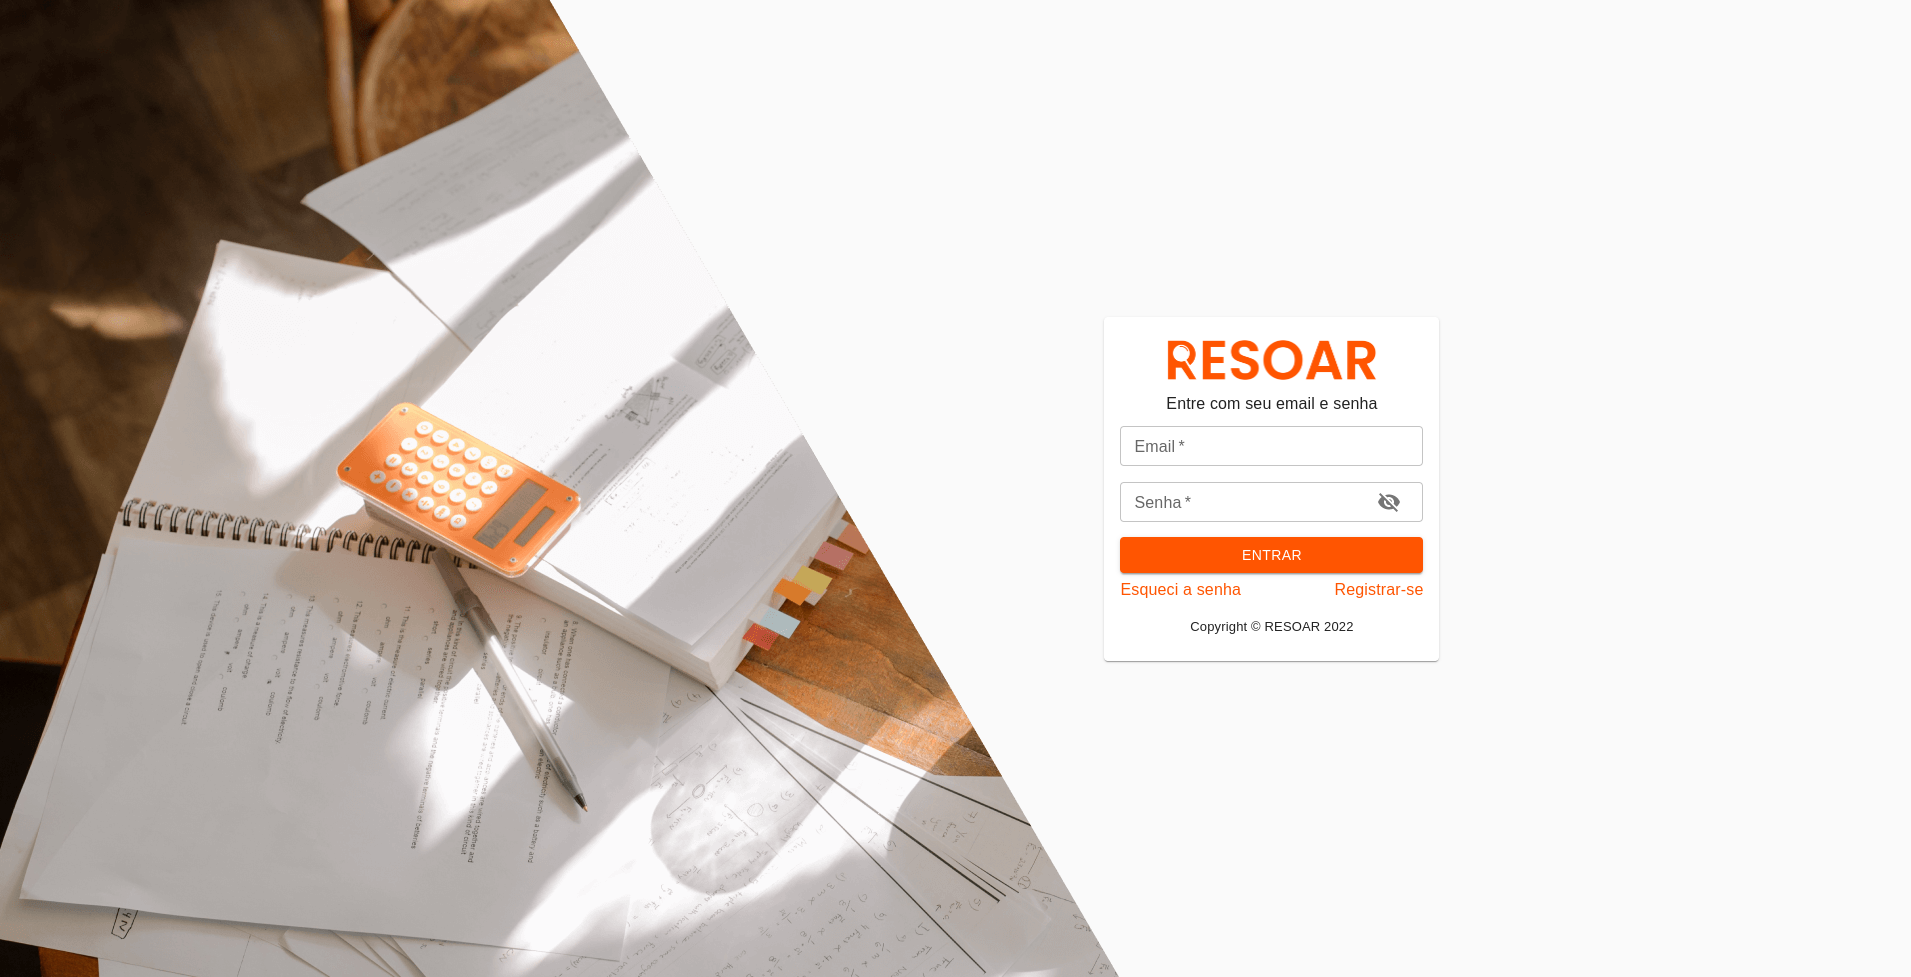
\includegraphics[scale=0.296]{img/resoar-login.png}}                                                                                                                                                                                                                                                           \\ \hline
    \end{tabular}
\end{table}

\begin{table}[H]
    \caption{Cadastro de usuário}
    \begin{tabular}{|p{1cm}|p{14cm}|}
        \hline
        \multicolumn{1}{|c|}{\textbf{02}} & \textbf{Cadastro de usuário}                                                                                                                                                                                   \\ \hline
        \multicolumn{2}{|l|}{\begin{tabular}[c]{@{}l@{}}\textbf{Como} novo usuário\\ \textbf{Eu quero} me cadastrar no sistema\\ \textbf{Para que} possa entrar no sistema.\end{tabular}}                                                                  \\ \hline
        \multicolumn{2}{|l|}{\textbf{Critérios de aceitação}}                                                                                                                                                                                              \\ \hline
        \multicolumn{2}{|l|}{\begin{tabular}[c]{@{}l@{}}1. Deve validar se já existe um usuário cadastrado com o mesmo email.\\2. Deve validar se os dois campos de senha são iguais.\\3. Deve solicitar a resolução de um desafio captcha. \end{tabular}} \\ \hline
        \multicolumn{2}{|c|}{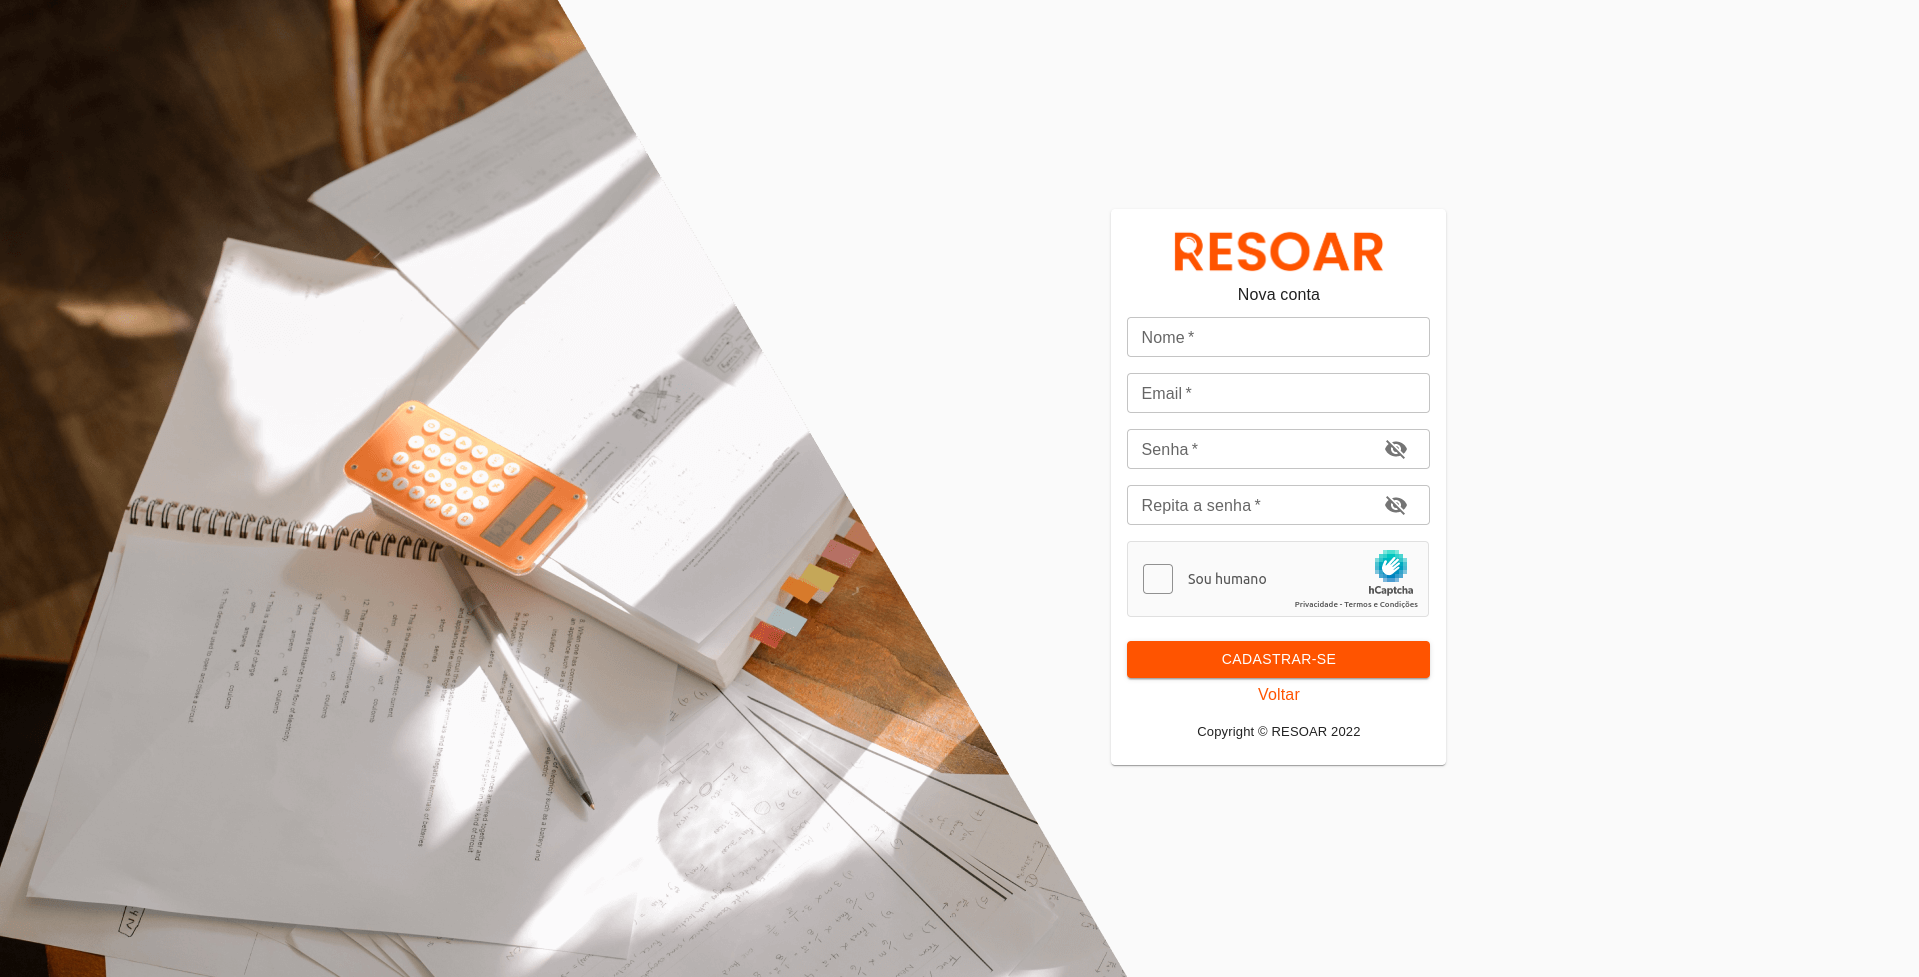
\includegraphics[scale=0.294]{img/resoar-new-account.png}}                                                                                                                                                                    \\ \hline
    \end{tabular}
\end{table}

\begin{table}[H]
    \caption{Recuperação de senha}
    \begin{tabular}{|p{1cm}|p{14cm}|}
        \hline
        \multicolumn{1}{|c|}{\textbf{03}} & \textbf{Recuperação de senha}                                                                                                                                                                                     \\ \hline
        \multicolumn{2}{|l|}{\begin{tabular}[c]{@{}l@{}}\textbf{Como} usuário do sistema\\ \textbf{Eu quero} poder solicitar um email de recuperação de senha\\ \textbf{Para que} possa criar uma nova senha para meu usuário.\end{tabular}}                  \\ \hline
        \multicolumn{2}{|l|}{\textbf{Critérios de aceitação}}                                                                                                                                                                                                 \\ \hline
        \multicolumn{2}{|l|}{\begin{tabular}[c]{@{}l@{}}1. Deve validar se o email informado existe no sistema.\\2. Deve enviar um email de recuperação, com validade máxima de 3 horas.\\3. Deve solicitar a resolução de um desafio captcha. \end{tabular}} \\ \hline
        \multicolumn{2}{|c|}{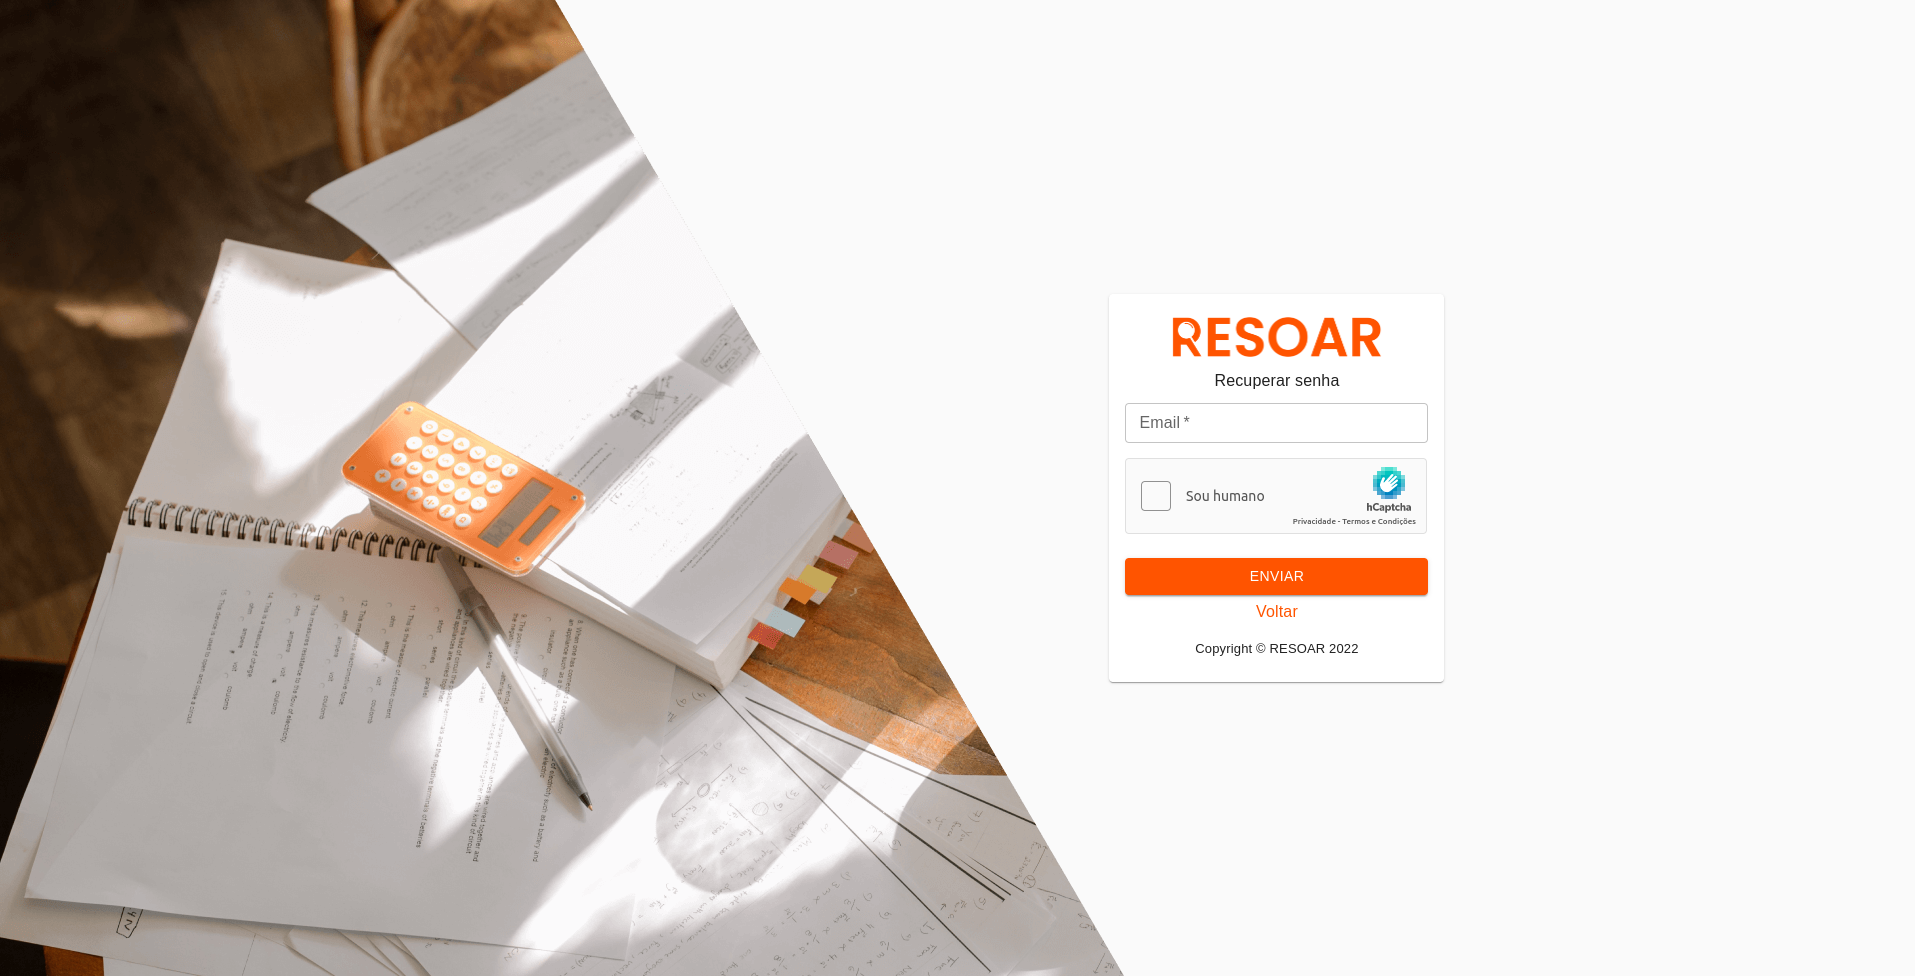
\includegraphics[scale=0.294]{img/resoar-password-recovery.png}}                                                                                                                                                                 \\ \hline
    \end{tabular}
\end{table}

\begin{table}[H]
    \caption{Visão geral}
    \begin{tabular}{|p{1cm}|p{14cm}|}
        \hline
        \multicolumn{1}{|c|}{\textbf{04}} & \textbf{Visão geral}                                                                                                                                                                                                                                                                            \\ \hline
        \multicolumn{2}{|l|}{\begin{tabular}[c]{@{}l@{}}\textbf{Como} usuário do sistema\\ \textbf{Eu quero} acessar uma tela de boas vindas ao entrar no sistema, contendo as\\ minhas publicações mais recentes, publicações salvas, e histórico de\\ publicações acessadas.\\ \textbf{Para que} tenha um ponto de partida.\end{tabular}} \\ \hline
        \multicolumn{2}{|l|}{\textbf{Critérios de aceitação}}                                                                                                                                                                                                                                                                               \\ \hline
        \multicolumn{2}{|l|}{\begin{tabular}[c]{@{}l@{}}1. Deve exibir ao menos as 3 ultimas publicações do usuário.\\2. Deve exibir ao menos as 3 ultimas publicações salvas para leitura.\\3. Deve exibir ao menos um histórico das 3 ultimas publicações acessadas. \end{tabular}}                                                       \\ \hline
        \multicolumn{2}{|c|}{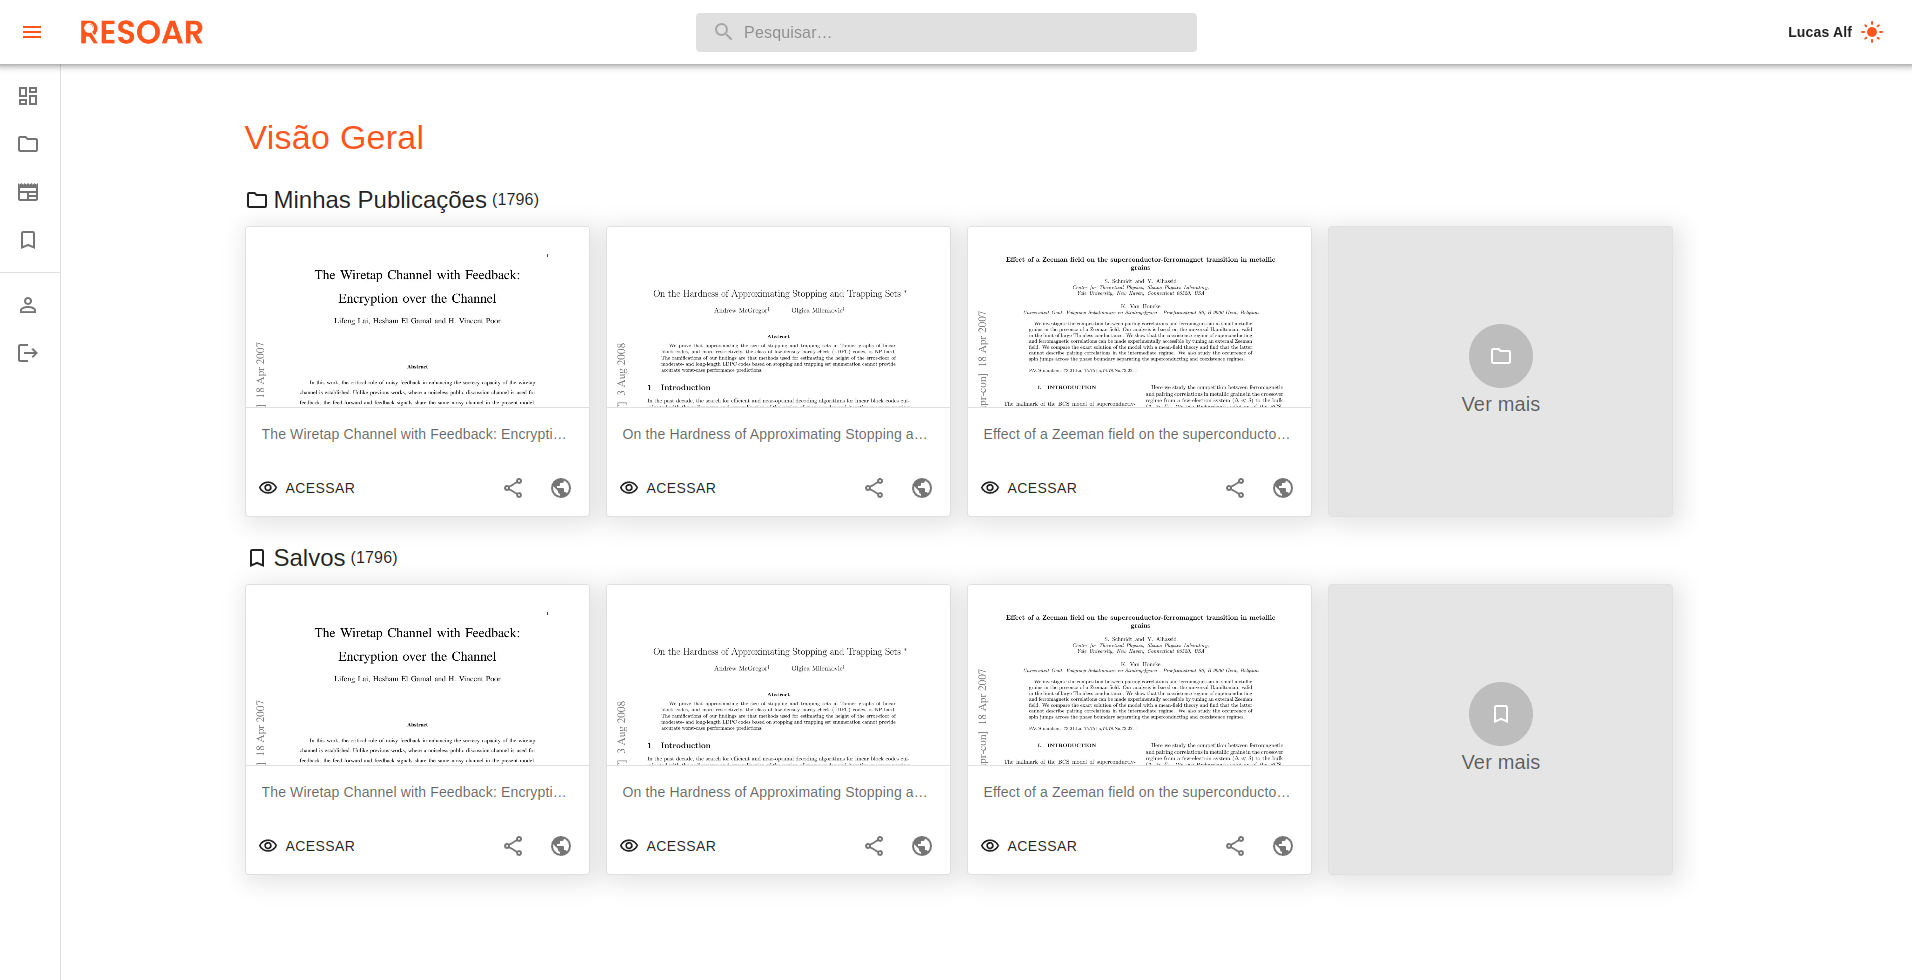
\includegraphics[scale=0.294]{img/resoar-overview.png}}                                                                                                                                                                                                                                                        \\ \hline
    \end{tabular}
\end{table}

\begin{table}[H]
    \caption{Minhas publicações}
    \begin{tabular}{|p{1cm}|p{14cm}|}
        \hline
        \multicolumn{1}{|c|}{\textbf{05}} & \textbf{Minhas publicações}                                                                                                                                                                                                                                                                                                                         \\ \hline
        \multicolumn{2}{|l|}{\begin{tabular}[c]{@{}l@{}}\textbf{Como} usuário do sistema\\ \textbf{Eu quero} acessar uma listagem contendo todas as minhas publicações\\ \textbf{Para que} possa navegar pelas publicações que realizei.\end{tabular}}                                                                                                                                          \\ \hline
        \multicolumn{2}{|l|}{\textbf{Critérios de aceitação}}                                                                                                                                                                                                                                                                                                                                   \\ \hline
        \multicolumn{2}{|l|}{\begin{tabular}[c]{@{}l@{}}1. Deve permitir a filtragem de publicações pelo título.\\2. Deve exibir na listagem o título, a imagem de capa, os autores, orientadores e\\ parte do resumo.\\3. Deve possuir um botão para a inclusão de nova publicação.\\4. Ao clicar em uma publicação, deve redirecionar para a página detalhada da\\ publicação. \end{tabular}} \\ \hline
        \multicolumn{2}{|c|}{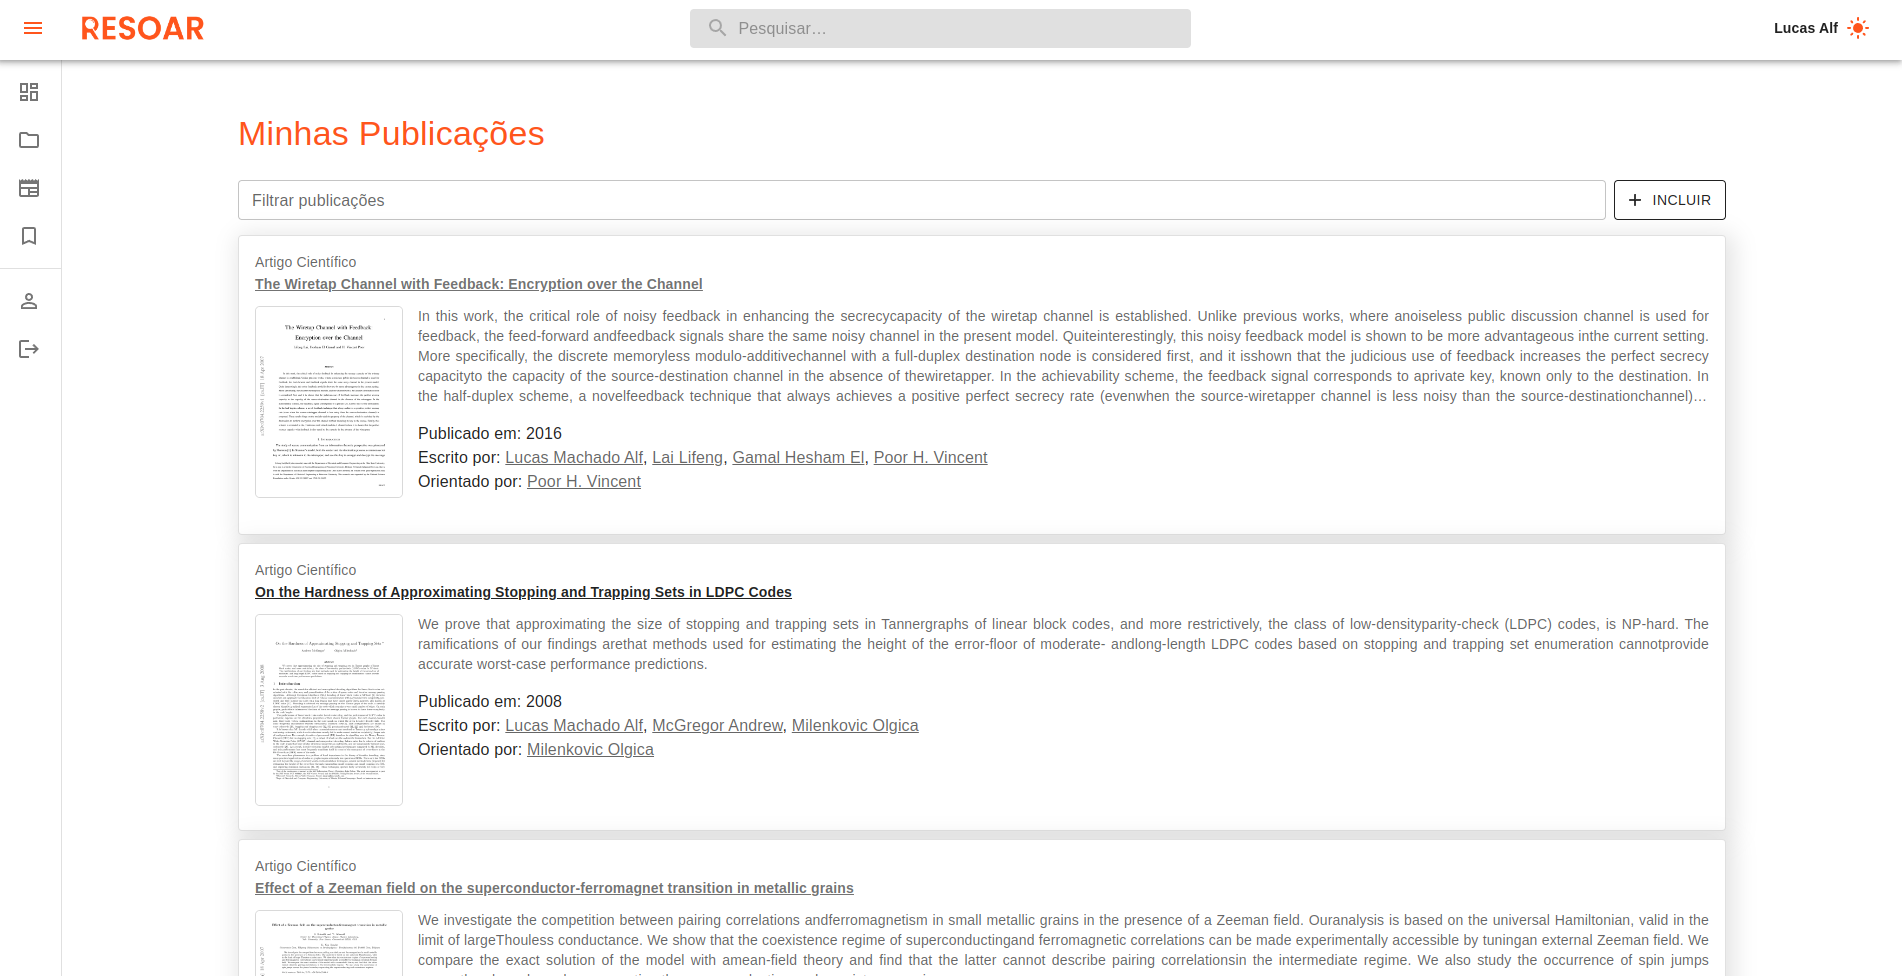
\includegraphics[scale=0.294]{img/resoar-my-research.png}}                                                                                                                                                                                                                                                                                                         \\ \hline
    \end{tabular}
\end{table}

\begin{table}[H]
    \caption{Nova publicação}
    \begin{tabular}{|p{1cm}|p{14cm}|}
        \hline
        \multicolumn{1}{|c|}{\textbf{06}} & \textbf{Nova publicação}                                                                                                                                                                                                                               \\ \hline
        \multicolumn{2}{|l|}{\begin{tabular}[c]{@{}l@{}}\textbf{Como} usuário do sistema\\ \textbf{Eu quero} realizar uma nova publicação\\ \textbf{Para que} possa salvar as minhas publicações no sistema.\end{tabular}}                                                                         \\ \hline
        \multicolumn{2}{|l|}{\textbf{Critérios de aceitação}}                                                                                                                                                                                                                                      \\ \hline
        \multicolumn{2}{|l|}{\begin{tabular}[c]{@{}l@{}}1. Deve solicitar os campos de título, resumo, ano, tipo, visibilidade, idioma,\\ instituição, autores, orientadores e arquivo da publicação.\\2. Dentro do campo de autores sempre deve haver no mínimo o próprio usuário. \end{tabular}} \\ \hline
        \multicolumn{2}{|c|}{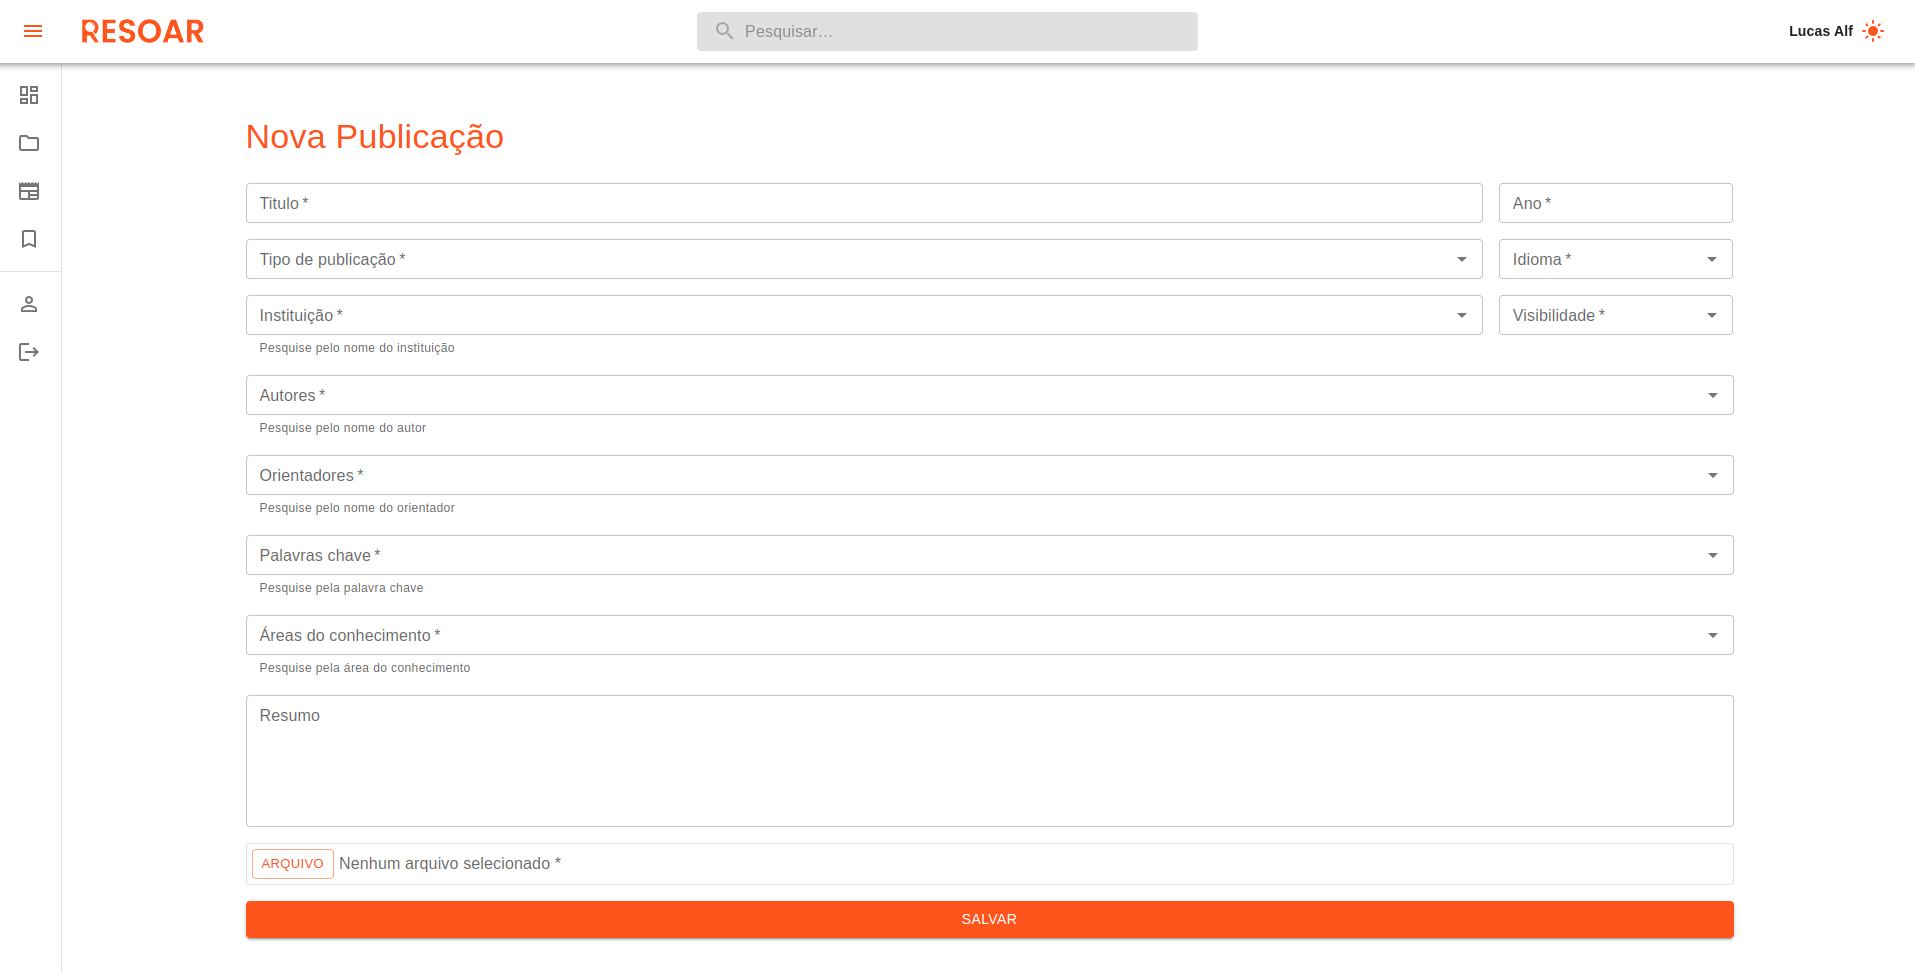
\includegraphics[scale=0.46]{img/resoar-add-research.png}}                                                                                                                                                                                                            \\ \hline
    \end{tabular}
\end{table}

\begin{table}[H]
    \caption{Pesquisar publicações}
    \begin{tabular}{|p{1cm}|p{14cm}|}
        \hline
        \multicolumn{1}{|c|}{\textbf{07}} & \textbf{Pesquisar publicações}                                                                                                                                                                                                                                           \\ \hline
        \multicolumn{2}{|l|}{\begin{tabular}[c]{@{}l@{}}\textbf{Como} usuário do sistema\\ \textbf{Eu quero} pesquisar por publicações, podendo utilizar de filtros \\ \textbf{Para que} possa encontrar as publicações que desejo visualizar.\end{tabular}}                                                         \\ \hline
        \multicolumn{2}{|l|}{\textbf{Critérios de aceitação}}                                                                                                                                                                                                                                                        \\ \hline
        \multicolumn{2}{|l|}{\begin{tabular}[c]{@{}l@{}}1. Deve permitir a busca por termos contidos dentro das publicações.\\2. Deve permitir a filtragem por ano, autor, orientador, tipo e idioma.\\3. Uma caixa de pesquisa por publicações sempre deve estar visível\\ na interface do usuário.  \end{tabular}} \\ \hline
        \multicolumn{2}{|c|}{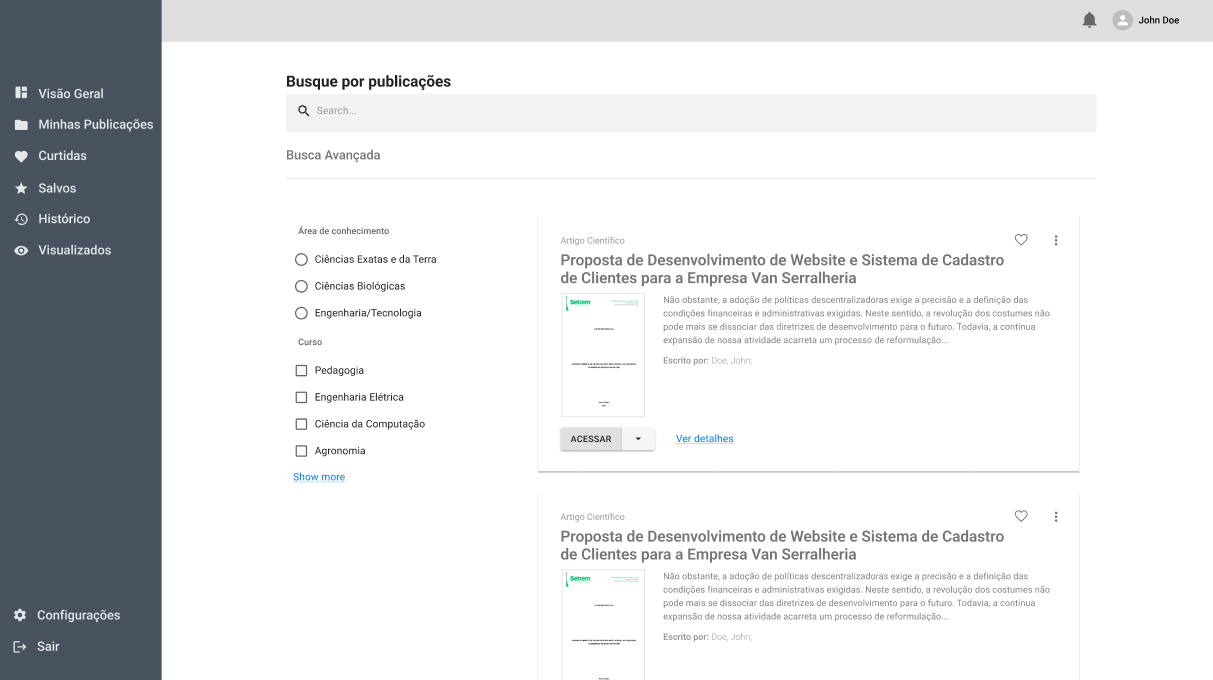
\includegraphics[scale=0.46]{img/resoar-search.png}}                                                                                                                                                                                                                                    \\ \hline
    \end{tabular}
\end{table}

\begin{table}[H]
    \caption{Visualizar publicação}
    \begin{tabular}{|p{1cm}|p{14cm}|}
        \hline
        \multicolumn{1}{|c|}{\textbf{08}} & \textbf{Visualizar publicação}                                                                                                                                                                                                                                                                                                                                                                       \\ \hline
        \multicolumn{2}{|l|}{\begin{tabular}[c]{@{}l@{}}\textbf{Como} usuário do sistema\\ \textbf{Eu quero} visualizar uma publicação \\ \textbf{Para que} possa ver os autores, orientadores, resumo e baixar o arquivo\\ da publicação.\end{tabular}}                                                                                                                                                                                         \\ \hline
        \multicolumn{2}{|l|}{\textbf{Critérios de aceitação}}                                                                                                                                                                                                                                                                                                                                                                                    \\ \hline
        \multicolumn{2}{|l|}{\begin{tabular}[c]{@{}l@{}}1. Deve exibir o título da publicação em destaque.\\2. Deve exibir a capa da publicação, e informações como os autores,\\ orientadores, tipo de publicação, idioma e resumo.\\3. Deve permitir realizar o \emph{download} da publicação.\\4. Deve permitir salvar a publicação para mais tarde.\\5. Deve permitir gerar um \emph{link} de compartilhamento da publicação. \end{tabular}} \\ \hline
        \multicolumn{2}{|c|}{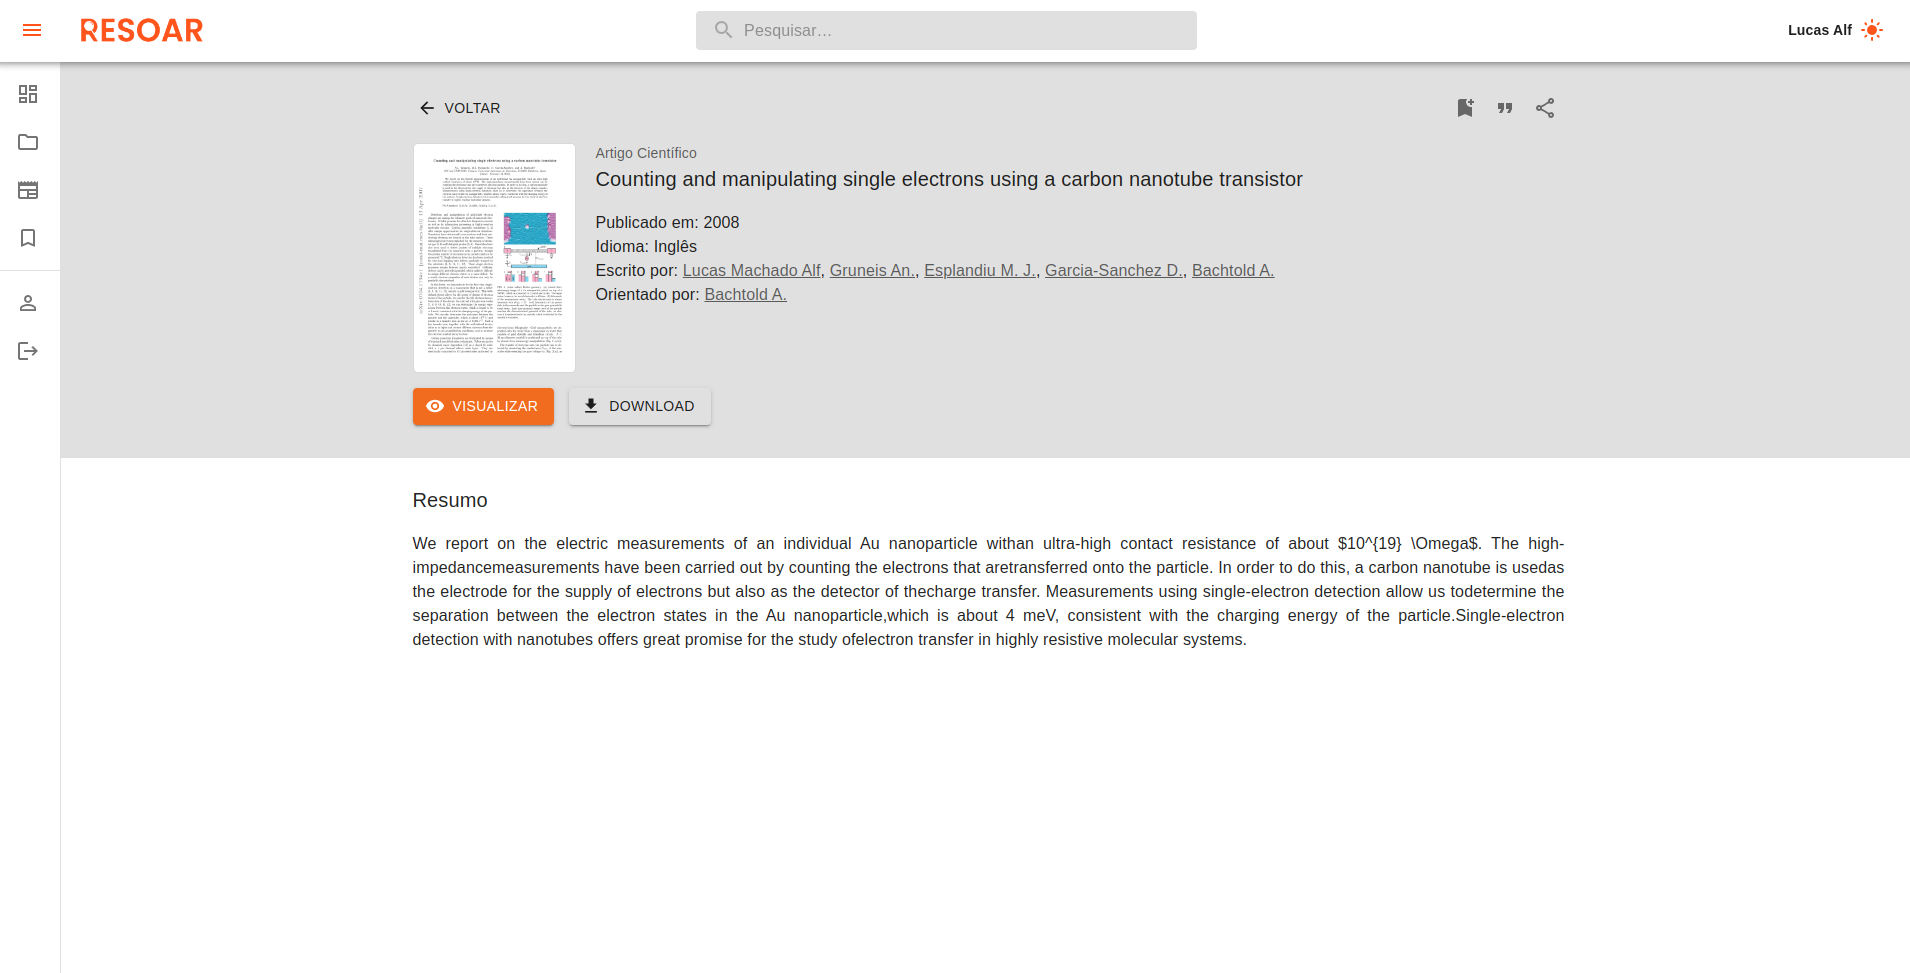
\includegraphics[scale=0.41]{img/resoar-view-research.png}}                                                                                                                                                                                                                                                                                                                                                         \\ \hline
    \end{tabular}
\end{table}

\begin{table}[H]
    \caption{Perfil do usuário}
    \begin{tabular}{|p{1cm}|p{14cm}|}
        \hline
        \multicolumn{1}{|c|}{\textbf{09}} & \textbf{Perfil do usuário}                                                                                                                                                                                                                                                  \\ \hline
        \multicolumn{2}{|l|}{\begin{tabular}[c]{@{}l@{}}\textbf{Como} usuário do sistema\\ \textbf{Eu quero} acessar uma página de perfil de usuário \\ \textbf{Para que} possa atualizar minhas informações, e trocar minha senha.\end{tabular}}                                                                       \\ \hline
        \multicolumn{2}{|l|}{\textbf{Critérios de aceitação}}                                                                                                                                                                                                                                                           \\ \hline
        \multicolumn{2}{|l|}{\begin{tabular}[c]{@{}l@{}}1. Deve exibir o nome e a foto do usuário.\\2. Deve listar as publicações as quais o usuário participa como autor.\\3. Caso o usuário esteja acessando o seu próprio perfil, devem existir opções\\ para editar as informações e trocar a senha. \end{tabular}} \\ \hline
        \multicolumn{2}{|c|}{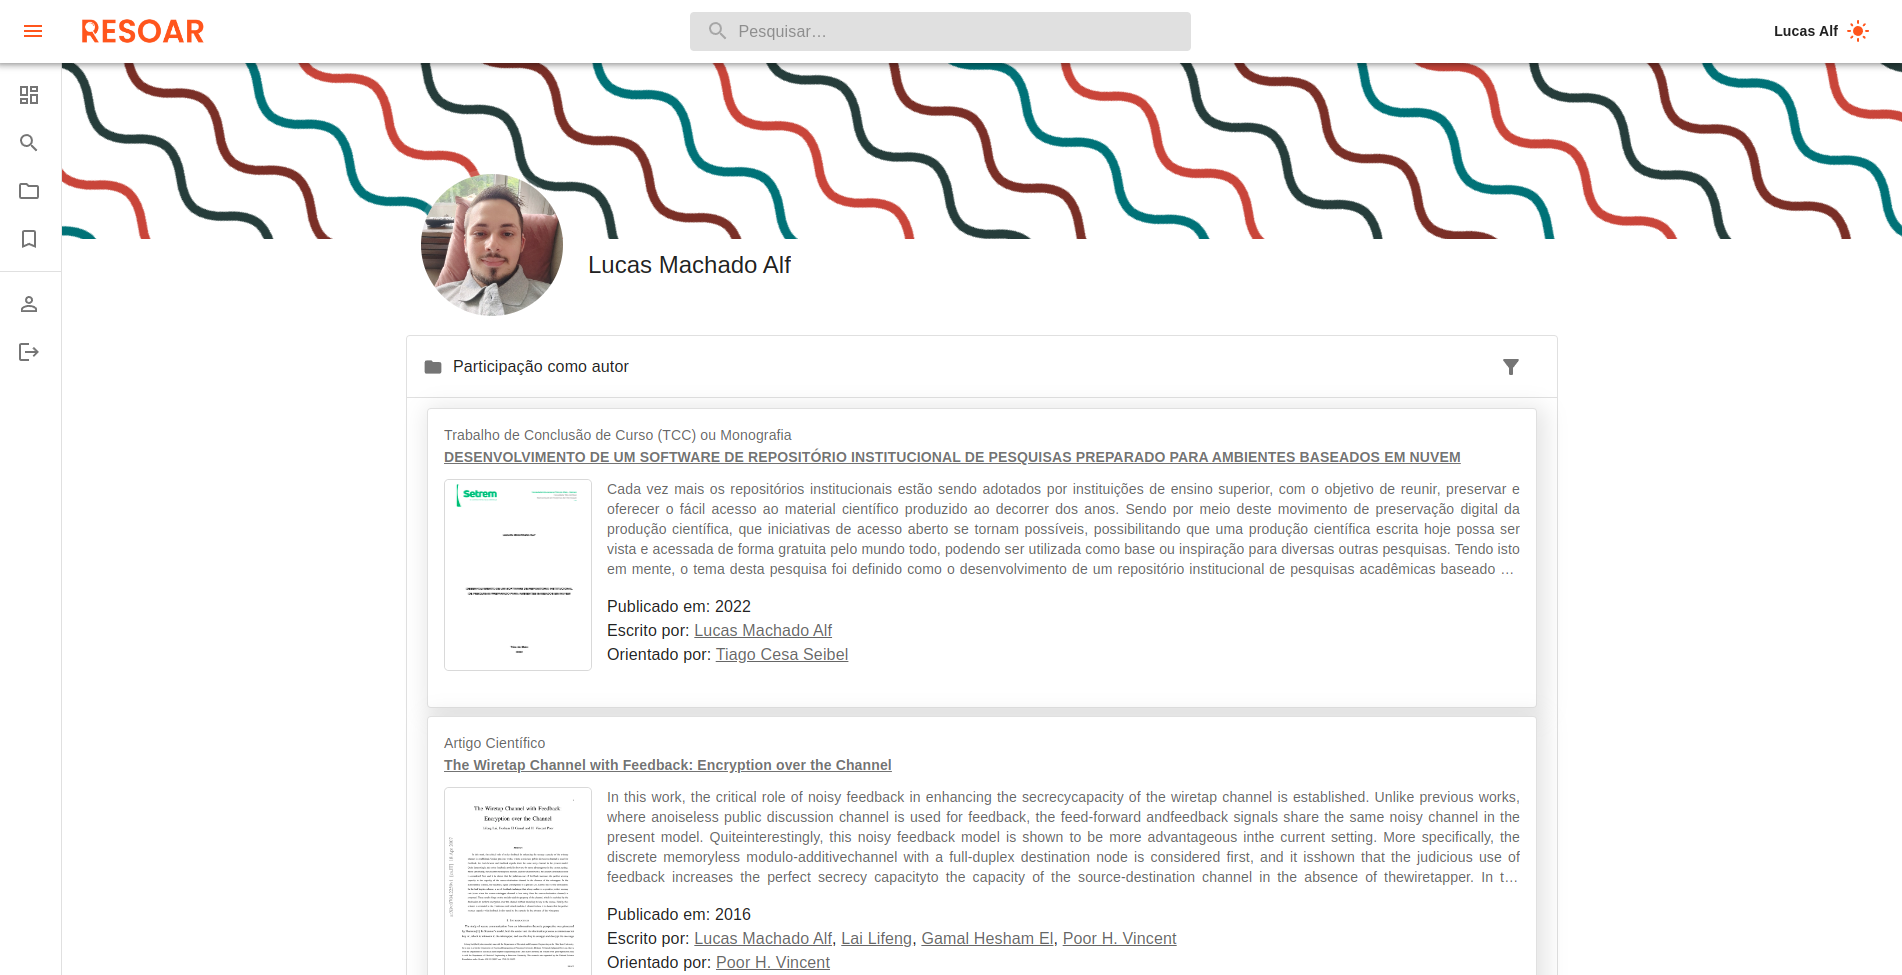
\includegraphics[scale=0.46]{img/resoar-account.png}}                                                                                                                                                                                                                                      \\ \hline
    \end{tabular}
\end{table}

% \chapter*{Conclusão} \label{chap:concl}

Cada vez mais os repositórios institucionais estão sendo adotados por instituições de
ensino superior, com o objetivo de reunir, preservar e oferecer o fácil acesso ao material
científico produzido ao decorrer dos anos. Sendo por meio deste movimento de preservação
digital da produção científica, que iniciativas de acesso aberto se tornam possíveis,
possibilitando que uma produção científica escrita hoje possa ser vista e acessada
de forma gratuita pelo mundo todo, podendo ser utilizada como base ou inspiração para
diversas outras pesquisas.

Também torna-se relevante a existência do desenvolvimento ativo de diferentes
alternativas de \emph{softwares} utilizados para elaborar tais repositórios
institucionais, tendo em vista o constante progresso tecnológico, e a necessidade
de que estas ferramentas não fiquem ultrapassadas ou monopolizadas por uma única
opção de \emph{software}. Além da necessidade da existência de padrões, para que
estas alternativas não criem um ambiente fragmentado de sistemas e padrões que não
são compatíveis entre si.

O objetivo deste trabalho de desenvolver um repositório institucional de pesquisas
acadêmicas baseado em nuvem, visando reunir e preservar as publicações acadêmicas
e científicas produzidas em âmbito universitário, além de unificar o processo
de publicações e correções por parte dos orientadores em uma única plataforma,
foi atingido, por meio do desenvolvimento de um novo \emph{software web} de
repositório institutional que foi denominado de \emph{RESOAR}
(\emph{Research Open Access Repository}).

O \emph{RESOAR} foi desenvolvido tendo como objetivo utilizar de tecnologias baseadas
em nuvem para realizar o armazenamento das publicações acadêmicas, possuindo suporte
a serviços de \emph{Object Storage} como o \emph{Amazon S3} e o \emph{Digital Ocean Spaces}.

Além disto, todas as configurações tanto do \emph{backend} quanto do \emph{frontend}
podem ser realizadas por meio de variáveis de ambiente, visando facilitar a implantação
do sistema em ambientes baseados em nuvem por meio de imagens \emph{docker}, tendo como
principio a ideia de nunca precisar acessar remotamente o container para realizar qualquer
tipo de configuração.

A primeira hipótese deste trabalho apresenta que "O recurso de \emph{Full Text Search} presente
no banco de dados PostgreSQL pode ser utilizado como uma alternativa viável para realizar
as consultas por publicações dentro do repositório acadêmico proposto, (menos de 1 segundo
por consulta), mesmo em bases de dados com mais de 3.500 publicações".

Esta primeira hipótese foi validada por meio da execução de testes de carga e estresse
sobre sobre o \emph{endpoint} de consulta por publicações do \emph{backend} desenvolvido.
Com os dados coletados, foi constatado que no cenário descrito pela hipótese, uma consulta
no repositório institucional possui um tempo médio de 114,54 milissegundos.

Já a segunda hipótese deste trabalho afirma que "O processo desenvolvido para extração do
texto das publicações durante o auto arquivamento é rápido o suficiente para não necessitar
de processamento em segundo plano (menos de 3 segundos), mesmo em publicações com mais de
12.000 palavras, cerca de 40 páginas de texto em português com fonte tamanho 12,
considerando que cada página tenha 300 palavras."

Esta segunda hipótese também foi validada por meio da aplicação de um teste de carga
e estresse sobre o \emph{backend} desenvolvido para o repositório institucional. Por meio
das métricas coletadas, foi constatado que uma publicação com as características
descritas pela hipótese, demora em média 2,30 segundos para ser concluída.

Em suma, o foco deste trabalho de desenvolver um novo repositório institucional
de pesquisas acadêmicas, utilizando de tecnologias baseadas em nuvem, e unificar
o processo de publicações e correções por parte dos alunos e orientadores, foi atingido.
Proporcionando aos envolvidos um grande aprendizado nas diversas áreas que envolvem
o desenvolvimento de \emph{software}, além de possibilitar a aplicação em prática dos
conhecimentos adquiridos ao decorrer da graduação.

Também fica como contribuição, a possibilidade da utilização do \emph{software}
desenvolvido, tanto pela SETREM, quanto a outras instituições que venham desenvolver
interesse pela utilização, ou pela contribuição com o projeto por meio de sugestões
ou melhorias ao \emph{software} de repositório institucional desenvolvido.

Como proposta futura, fica a sugestão da criação de um recurso dentro do próprio
repositório institucional, que permita realizar anotações em cima das publicações
acadêmicas, como a adição de comentários ou rabiscos de caneta. Este recurso poderia
ser especialmente útil para os orientadores, que poderiam adicionar sugestões ou
correções as pesquisas dentro da própria plataforma. No momento em que este trabalho
foi desenvolvido, foram encontradas poucas bibliotecas que permitem este tipo de
edição diretamente pelo o navegador do usuário, sendo em maioria pagas,
inviabilizando a aplicação do recurso no sistema.


%\bibliographystyle{template/abnt}
%% para português
\bibliographystyle{template/abnt-pt}
\bibliography{bib/bibliography}

\end{document}
